\chapter{HASIL DAN PEMBAHASAN}
\label{bab4}

% Ubah bagian-bagian berikut dengan isi dari pengujian dan analisis

Pada bab ini dipaparkan hasil dan analisa dari pelaksanaan skenario tahap  metodologi, skenario pengujian dan evaluasi pengujiannya. Pengujian dan evaluasi dilakukan guna mengetahui tingkat kesalahan dalam metodologi serta analisis hasil yang didapatkan untuk mencapai kesimpulan. Tahapan skenario yang dilaksanakan sebagai berikut :

% \begin{enumerate}
%   \item Pengujian akurasi model dalam beberapa situasi
%   \item Pengujian interaksi model pada beberapa responden
%   \item Pengujian pada robot dengan beberapa kondisi
% \end{enumerate}
% Dengan hasil metodologi serta pelaksanaan skenario-skenario pengujian yang dipaparkan pada bab Penelitian dan pembahasan, diharapkan mendapatkan hasil dan analisa sehingga dapatditarik kesimpulan dari pelaksanaan tugas akhir ini.

% \section{Hasil metodologi}
% Pada metodologi terdapat blok diagaram sebagai acuan dalam Penelitian yang telah dilaksanakan. Adapun hasil dari blok diagram tersebut secara rinci sebagai berikut :

\section{Hasil Metodologi}
Pada bagian metodologi terdapat blok diagram dan telah dilakukan pelaksanaan Tugas Akhir sesuai dengan blok diagram tersebut. Adapun hasil dari tiap tahapan yang dilakukan pada blok diagram tersebut secara rinci sebagai berikut.

\subsection{Dataset}

\begin{table}[H]
  \centering
  \caption{Citra hasil dataset}
  \label{tab:citradaset}
  \begin{tabular}{|c|c|}
    \hline
    Pose   & Citra \\ \hline
    Diam   & 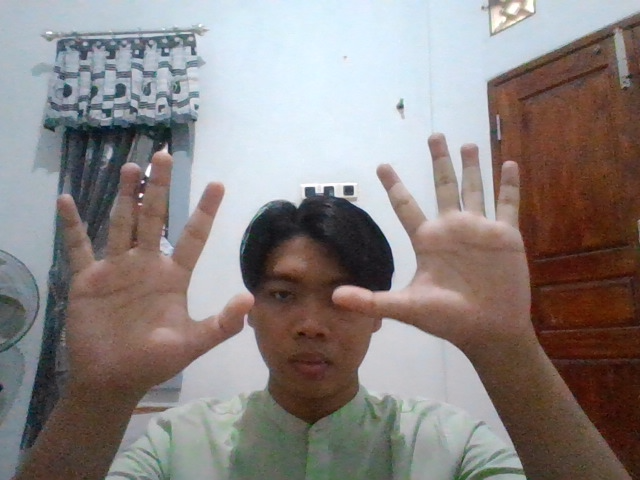
\includegraphics[width=0.4\linewidth]{../Gambar/posediam.png} \\ \hline
    Kanan  & 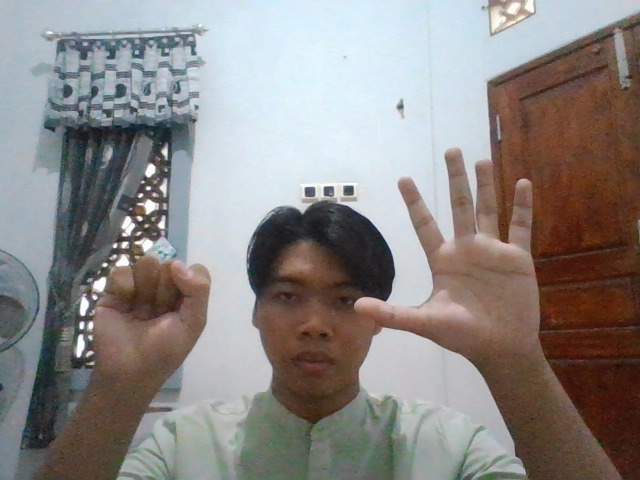
\includegraphics[width=0.4\linewidth]{../Gambar/posekanan.png} \\ \hline
    % Kiri   & 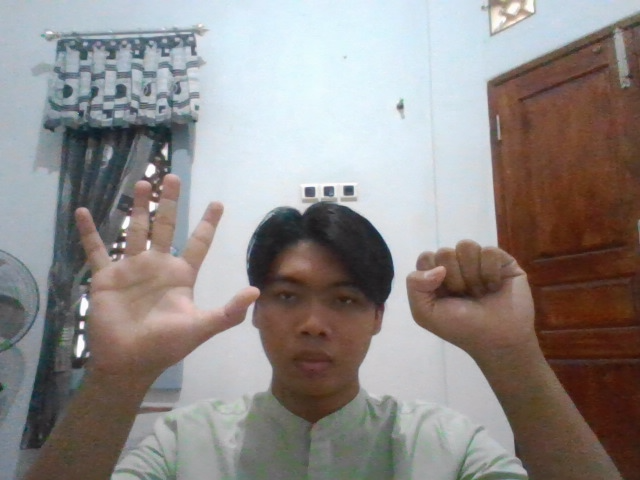
\includegraphics[width=0.4\linewidth]{../Gambar/posekiri.png} \\ \hline
    % Maju   & 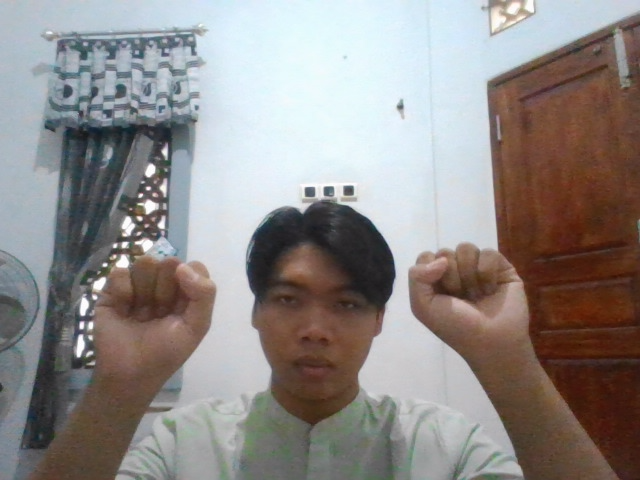
\includegraphics[width=0.5\linewidth]{../Gambar/posemaju.png} \\ \hline
    % Mundur & 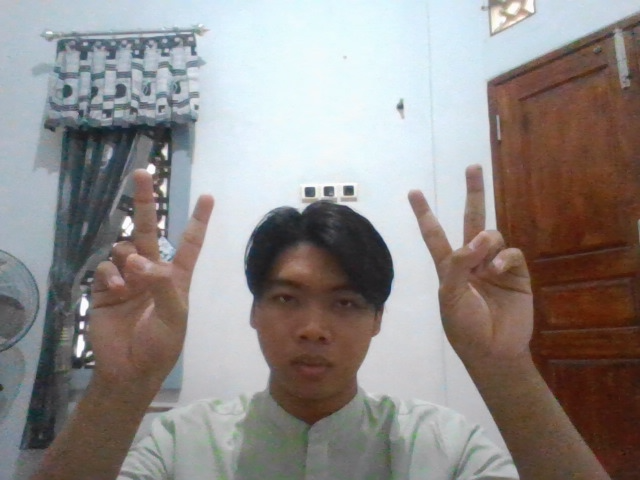
\includegraphics[width=0.5\linewidth]{../Gambar/posemundur.png} \\ \hline
  \end{tabular}
\end{table}

\begin{table}[H]
  \centering
  \begin{tabular}{|c|c|}
    \hline
    Pose   & Citra \\ \hline
    % Diam   & 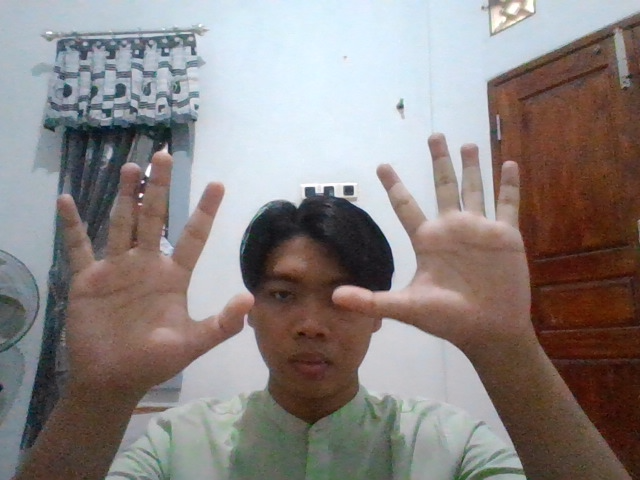
\includegraphics[width=0.4\linewidth]{../Gambar/posediam.png} \\ \hline
    % Kanan  & 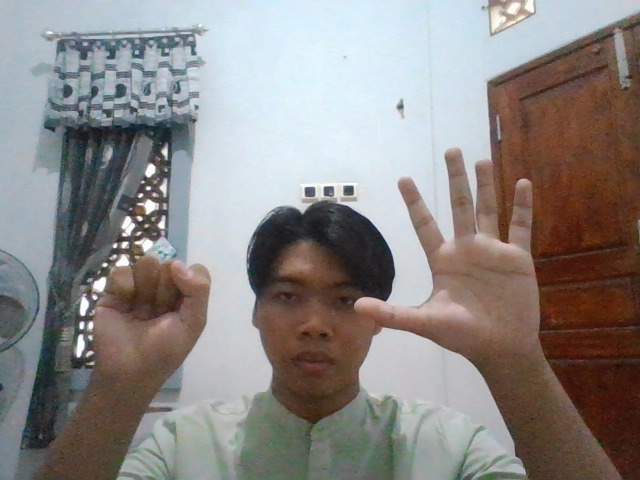
\includegraphics[width=0.4\linewidth]{../Gambar/posekanan.png} \\ \hline
    Kiri   & 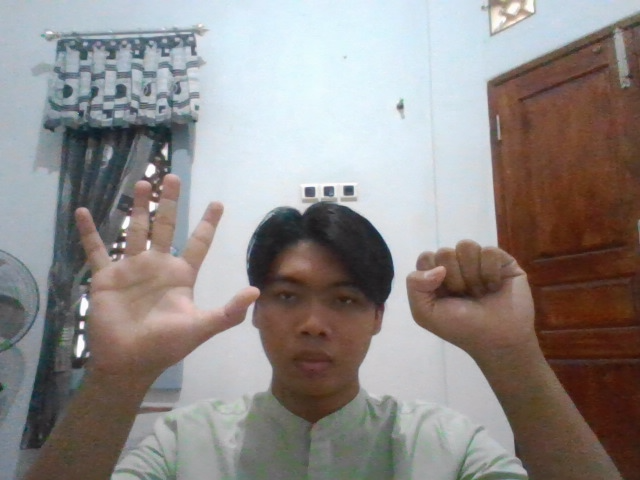
\includegraphics[width=0.4\linewidth]{../Gambar/posekiri.png} \\ \hline
    Maju   & 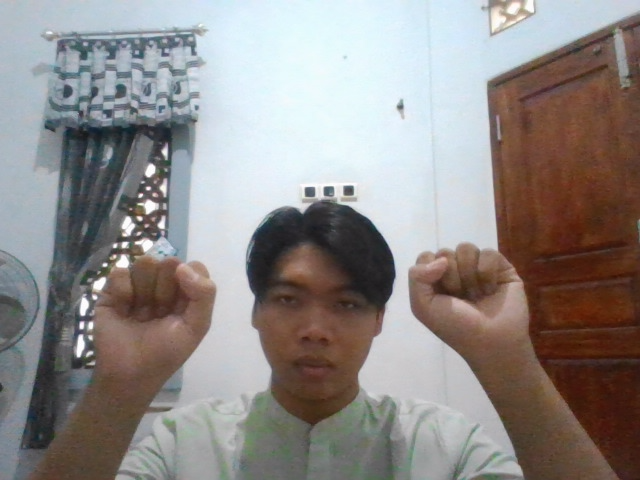
\includegraphics[width=0.4\linewidth]{../Gambar/posemaju.png} \\ \hline
    Mundur & 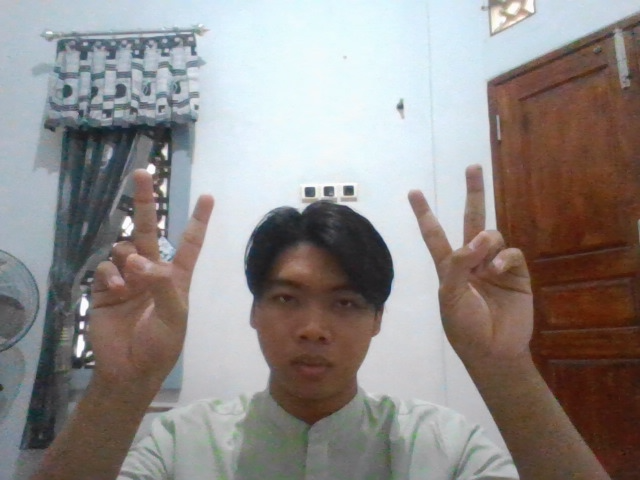
\includegraphics[width=0.4\linewidth]{../Gambar/posemundur.png} \\ \hline
  \end{tabular}
\end{table}

Proses pengumpulan dataset dilakukan dengan pengambilan citra menggunakan kamera. Hasil kamera berupa vidio yang selanjutnya dipotong menjadi citra. Pada tiap satu detik vidio akan dipotong menjadi 5 citra atau dapat dibilang sebagai 5 fps (\emph{frame per second}). Proses pengambilan citra dilakukan selama beberapa waktu untuk mendapatkan jumlah citra yang diinginkan pada tiap kelas. Citra yang dihasilkan merupakan citra berwarna dengan ukuran lebar 640 \emph{pixels} dan tinggi 480 \emph{pixels}. Proses tersebut dilakukan selama beberapa waktu untuk dapat mendapatkan beberapa frame citra untuk suatu kelas dan diulang kembali dengan kelas yang berbeda sampai seluruh kelas terpenuhi. Seluruh citra tangan diambil dari satu orang yang sama dan menggunakan jarak pengambilan antara 40cm sampai 60cm, yaitu jarak antara kamera dan tangan. Dalam proses pengambilan citra dilakukan beberapa variasi dalam pose tangan yaitu dengan sedikit merotasikan tangan dan sedikit menggerakkan tangan. Hal ini dilakukan agar tiap kelas memiliki variasi pose dan dapat mendeteksi dari berbagai kondisi pose. Adapun pose yang digunakan sebagai dataset dapat dilihat pada Tabel \ref{tab:citradaset}.



\subsection{Estimasi Pose}

\begin{figure}[H]
  \centering
  \begin{subfigure}{0.7\linewidth}
    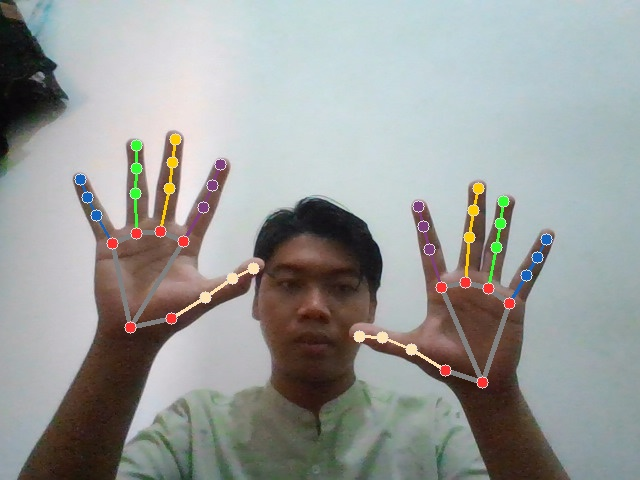
\includegraphics[width=\linewidth]{../Gambar/Cobak17.jpg}
    \caption{Citra hasil dataset}
    \label{fig:handlandmarkcitradataset}
  \end{subfigure}
  \begin{subfigure}{0.7\linewidth}
    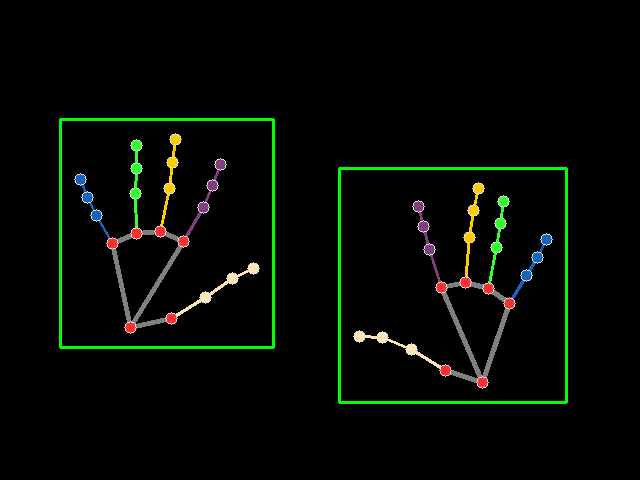
\includegraphics[width=\linewidth]{../Gambar/Cobak17.png}
    \caption{Citra hasil ektraksi fitur}
    \label{fig:handlandmarkcitraektraksi}
  \end{subfigure}
  \caption{Hasil \emph{hand landmark} serta \emph{bounding box}}
  \label{fig:hasilposepred}
\end{figure}

Proses estimasi pose dilakukan dengan menggambar \emph{hand landmark} yang telah terdeteksi dengan menggunakan \emph{Mediapipe} pada tiap-tiap citra yang telah dikumpulan pada tahap pengumpulan dataset. Proses menggambar \emph{hand landmark} dikelola oleh \emph{Mediapipe}. Proses yang dilakukan \emph{Mediapipe} untuk menggambar \emph{hand landmark} diawali dengan mendeteksi telapak tangan kemudian mencari titik-titik \emph{keypoint} lainnya. Jumlah \emph{keypoint} yang membentuk \emph{hand landmark} berjumlah 21 titik pada satu tangan, maka pada citra hasil deteksi akan dicari 42 titik dikarenakan mencari titik \emph{keypoint} dari kedua tangan. Setelah 21 titik pada masing-masing tangan ditemukan, selanjutnya yang dilakukan adalah menggambar \emph{hand landmark} pada masing-masing tangan yang telah ditemukan. Setelah \emph{hand landmark} telah digambar maka tiap-tiap \emph{hand landmark} digambar kembali pada citra berlatar hitam. Proses menggambar ulang \emph{hand landmark} dinamakan sebagai ekstraksi pose dan citra berlatar hitam dengan \emph{hand landmark} dinamakan sebagai citra ekstraksi pose. \emph{Hand landmark} pada citra hasil ektraksi pose memiliki bentuk serta ukuran yang sama seperti yang terdapat pada citra hasil dataset. Bentuk dan ukuran dari \emph{hand landmark} pada citra hasil ektraksi pose didapatkan dari titik-titik \emph{keypoint} yang yang telah terdeteksi pada citra hasil dataset. Pada citra ektraksi pose dibuat \emph{bounding box} yang mengecakup masing-masing \emph{hand landmark}. Ukuran \emph{bounding box} dibuat dari nilai koordinat terkecil pada sumbu x dan sumbu y serta nilai koordinat terbesar pada sumbu x dan sumbu y. Koordinat yang dimaksud merupakan koordinat dari hasil \emph{keypoint Mediapipe} yang masing-masing \emph{keypoint} memiliki koordinat pada sumbu x, y, dan z. Koordinat x dan y digunakan untuk membuat kotak \emph{bounding box} yang mencakup keseluruhan \emph{hand landmark} pada masing-masing tangan. Pada nilai koordinat terkecil akan dikurangi dengan 20 \emph{pixels} dan nilai koordinat terbesar akan ditambah dengan 20 \emph{pixels}. Penambahan serta pengurangan koordinat digunakan untuk mencakup keseluruhan \emph{hand landmark} yang telah dibuat. Penambahan dan pengurangan nilai koordinat terjadi karena tanpa adanya penambahan dan pengurangan nilai koordinat pada pembuatan \emph{bounding box} menyebabkan terdapat \emph{hand landmark} yang terpotong pada nilai \emph{keypoint} terbesar dan terkecil. Citra dengan \emph{hand landmark} didalamnya dapat dilihat pada Gambar \ref{fig:hasilposepred} dengan rincian Gambar \ref{fig:handlandmarkcitraektraksi} merupakan citra dataset yang telah terdapat \emph{hand landmark} dari \emph{Mediapipe} dan Gambar \ref{fig:handlandmarkcitraektraksi} merupakan citra ekstraksi fitur yang terdapat \emph{hand landmark} dan \emph{bounding box} didalamnya. 

\begin{table}[H]
  \centering
  \caption{Hasil posisi citra hasil transformasi}
  \label{tab:posisigtangan}
  \begin{tabular}{|c|c|c|}
  \hline
  Pose   &Pose Benar&Pose Terbalik\\ \hline
  Diam   & 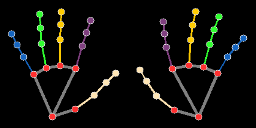
\includegraphics[width=0.4\linewidth]{../Gambar/Diam (1).png} & 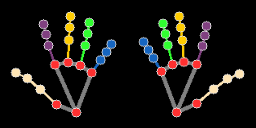
\includegraphics[width=0.4\linewidth]{../Gambar/DiamI (1).png} \\ \hline
  Kanan  & 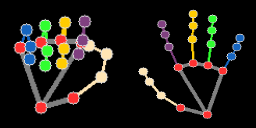
\includegraphics[width=0.4\linewidth]{../Gambar/Kanan (1).png} & 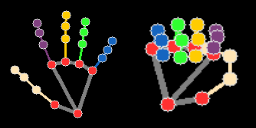
\includegraphics[width=0.4\linewidth]{../Gambar/KananI (1).png} \\ \hline
  Kiri   & 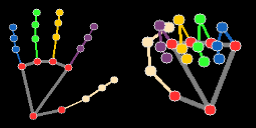
\includegraphics[width=0.4\linewidth]{../Gambar/Kiri (1).png} & 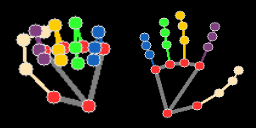
\includegraphics[width=0.4\linewidth]{../Gambar/KiriI (1).png} \\ \hline
  % Maju   & 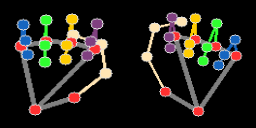
\includegraphics[width=0.4\linewidth]{../Gambar/Maju (1).png} & 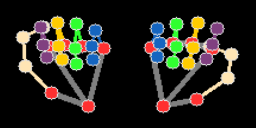
\includegraphics[width=0.4\linewidth]{../Gambar/MajuI (1).png} \\ \hline
  % Mundur & 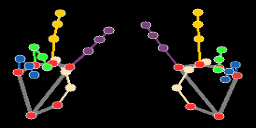
\includegraphics[width=0.4\linewidth]{../Gambar/Mundur (1).png} & 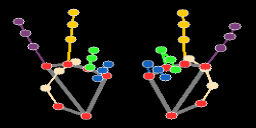
\includegraphics[width=0.4\linewidth]{../Gambar/MundurI (1).png} \\ \hline
  \end{tabular}
\end{table}

\begin{table}[H]
  \centering
  % \caption{Hasil posisi hand localization}
  % \label{tab:posisigtangan}
  \begin{tabular}{|c|c|c|}
  \hline
  Pose   &Pose Benar&Pose Terbalik\\ \hline
  % Diam   & 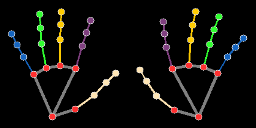
\includegraphics[width=0.4\linewidth]{../Gambar/Diam (1).png} & 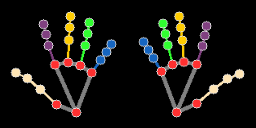
\includegraphics[width=0.4\linewidth]{../Gambar/DiamI (1).png} \\ \hline
  % Kanan  & 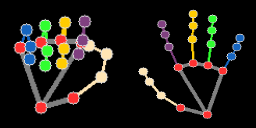
\includegraphics[width=0.4\linewidth]{../Gambar/Kanan (1).png} & 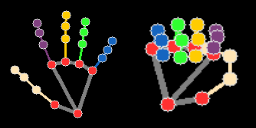
\includegraphics[width=0.4\linewidth]{../Gambar/KananI (1).png} \\ \hline
  % Kiri   & 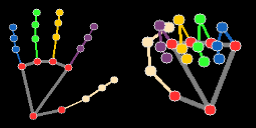
\includegraphics[width=0.4\linewidth]{../Gambar/Kiri (1).png} & 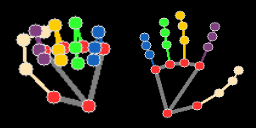
\includegraphics[width=0.4\linewidth]{../Gambar/KiriI (1).png} \\ \hline
  Maju   & 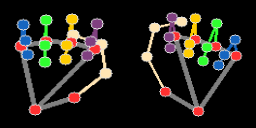
\includegraphics[width=0.4\linewidth]{../Gambar/Maju (1).png} & 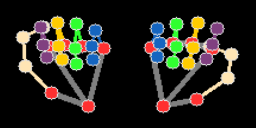
\includegraphics[width=0.4\linewidth]{../Gambar/MajuI (1).png} \\ \hline
  Mundur & 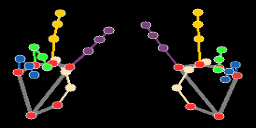
\includegraphics[width=0.4\linewidth]{../Gambar/Mundur (1).png} & 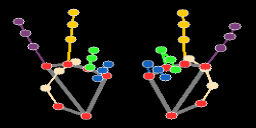
\includegraphics[width=0.4\linewidth]{../Gambar/MundurI (1).png} \\ \hline
  \end{tabular}
\end{table}

Citra hasil ektraksi pose yang terdapat \emph{bounding box} didalamnya diolah kembali dengan cara membuang citra diluar \emph{bounding box}. Citra ekstraksi fitur dipotong sesuai ukuran bounding pada masing-masing \emph{hand landmark}. Pada masing-masing \emph{bounding box} yang telah dipotong dilakukan pengubahan ukuran menjadi lebar 128 \emph{pixels} dan tinggi 128 \emph{pixels}. Pengubahan ukuran digunakan untuk menyamakan ukuran dari kedua \emph{bounding box} pada satu citra. Setelah ukuran sama maka dilakukan penumpukan secara horizontal pada kedua \emph{bounding box} didalam satu citra. Dari hasil penumpukan ini terdapat dua hasil yaitu posisi benar dan posisi terbalik. Perbedaaan posisi diakibatkan oleh proses pendeteksian tangan oleh \emph{Mediapipe} dan proses penumpukan citra setelah citra dipotong seukuran \emph{bounding box}. Posisi benar adalah disaat tangan kanan yang terdeteksi terlebih dahulu begitu sebaliknya pada posisi terbalik yaitu disaat tangan kiri terdeteksi terlebih dahulu oleh \emph{Mediapipe}. Posisi benar merupakan posisi \emph{hand landmark} tangan kanan berada pada posisi kanan citra. Sebaliknya posisi terbalik merupakan posisi \emph{hand landmark} tangan kanan berada pada posisi kiri citra sedangkan posisi kanan ditempati oleh \emph{hand landmark} tangan kiri. Hasil dari penumpukan citra menyebabkan perubahan pada citra ekstraksi fitur pada awalnya berukuran lebar 640 \emph{pixels} dan tinggi 480 \emph{pixels} menjadi lebar 256 \emph{pixels} dan tinggai 128 \emph{pixels}. Citra hasil penumpukan dan posisi yang dihasilkan dapat dilihat pada Tabel \ref{tab:posisigtangan}.





\subsection{Klasifikasi}
Proses klasifikasi dimulai dari \emph{training} dataset. Sebelum melakukan \emph{training} maka dibutuhkannya data citra pada tiap kelas. Tiap kelas memiliki \emph{train data} dan \emph{validation data}. Data-data ini diambil dari proses sebelumnya yaitu citra yang telah melewati tahap estimasi pose. Citra untuk \emph{training} data pada tiap kelas berjumlah 500 dengan rincian 250 citra posisi benar dan 250 citra posisi terbalik, sedangkan citra untuk \emph{validation data} berjumlah 80 citra dengan 40 citra posisi benar dan 40 citra posisi invers. Keseluruhan citra yang digunakan utnuk \emph{training} dan \emph{validation} berjumlah 2500 citra untuk \emph{training} dan 480 citra untuk \emph{validation}. Tabel pesebaran data citra tiap kelas dapat dilihat pada Tabel \ref{tab:tiapkelas}. 

\begin{table}[H]
  \centering
  \caption{Jumlah Citra Tiap kelas}
  \label{tab:tiapkelas}
  \begin{tabular}{|c|c|c|}
  \hline
  kelas  & \emph{Training} Data & \emph{Validation} Data \\ \hline
  Diam   & 500        & 80              \\ \hline
  Kanan  & 500        & 80              \\ \hline
  Kiri   & 500        & 80              \\ \hline
  Maju   & 500        & 80              \\ \hline
  Mundur & 500        & 80              \\ \hline
  \end{tabular}
\end{table}

Metode \emph{training} yang digunakan adalah CNN dengan urutan seperti pada Gambar \ref{fig:layerCNn}. Training dimulai dengan dilakukannya konvolusi pada input citra yang berukuran lebar 256 \emph{pixels} dan tinggai 128 \emph{pixels}. Konvolusi menggunakan ukuran \emph{filter} 3x3 dan berjumlah 64 \emph{filter}. Pada tahapan konvolusi pertama diberikan padding yang menyebabkan tidak berkurangnya ukuran citra, maka ukuran citra hasil konvolusi pertama tetap berukuran lebar 256 \emph{pixels} dan tinggai 128 \emph{pixels} namun dengan jumlah \emph{layer} 64. Setelah konvolusi dilakukan \emph{pooling}, metode \emph{pooling} yang digunakan adalah \emph{max pooling} dengan ukuran \emph{filter} 2x2 yang menyebabkan perubahan pada ukuran citra. Perubahan yang terjadi pada ukuran citra menjadi setengah dari ukuran awal yaitu menjadi lebar 128 \emph{pixels} dan tinggi 64 \emph{pixels}. Setelah dilakukan \emph{max pooling} tahap selanjutnya dilakukan konvolusi kembali. Konvolusi kedua dilakukan dengan ukuran \emph{filter} yang smaa yaitu 3x3 dan kembali digunakan padding yang menyebabkan ukuran citra tidak berubah. Pada konvolusi kedua jumlah \emph{filter} yang digunakan adalah setengah dari jumlah \emph{filter} pada konvolusi pertama yaitu berjumlah 32 \emph{layer}. Tahap konvolusi kedua menghasilkan ukuran citra yang tetap yaitu lebar 128 \emph{pixels} dan tinggi 64 \emph{pixels} dengan jumlah \emph{filter} 32. Setelah konvolusi kedua dilakukan max \emph{pooling} kembali dengan filter 2x2 yang menyebabkan ukuran citra menjadi setengah dari ukuran hasil konvolusi kedua. Hasil citra dari \emph{pooling} kedua yaitu lebar 64 \emph{pixels} dan tinggi 32 \emph{pixels} dengan jumlah \emph{layer} yaitu 32. Citra hasil dari \emph{pooling} kedua diubah menjadi vektor pada layer \emph{flatten}. hasil vektor digunakan untuk perhitungan menggunakan metode \emph{neuron network} dan menghasilkan output lima kelas. Setelah di tentukannya konfigurasi layer CNN maka tahapan selanjutnya yaitu konfigurasi hyperparameter. Adapun konfigurasi pada hyperparameter yang digunakan dapat dilihat pada Tabel \ref{fig:hyperparameter} berikut. Citra yang digunakan sebagai data pada saat \emph{training} dan \emph{validation} berukuran 256x128 yang merupakan citra hasil ekstraksi fitur. Jumlah total dari image yang digunakan untuk \emph{training} berjumlah 2400 citra. 2500 citra tersebut tidak memungkingkan untuk langsung di \emph{training} pada sekali \emph{epoch} maka dari itu citra dibagi menjadi beberapa step per epoch dan \emph{batchsize}. Tiap step per epoch akan menggunakan 32 citra, jumlah step per epoch ini selanjutnya dipanggil sebagai \emph{batchsize}. Alasan penggunaan batchsize dengan nilai 32 untuk mengurangi beban pada laptop pada saat dilakukan \emph{training}. Tiap step per epoch menggunakan 32 citra maka dibutuhkan 78 step per epoch pada sekali \emph{epoch}, 78 step per epoch ini selanjutnya di sebut sebagai step per epoch.


\begin{table}[H]
  \centering
  \caption{Konfigurasi \emph{hyperparameter}}
  \label{fig:hyperparameter}
  \begin{tabular}{|c|c|lll}
  \cline{1-2}
  \emph{Hyperparameter} & Konfigurasi \\ \cline{1-2}
  Epochs         & 5 \\ \cline{1-2}
  Batchsize      & 32 \\ \cline{1-2}
  Step per epoch      & 78 \\ \cline{1-2}
  Optimizer      & Adam \\ \cline{1-2}
  \end{tabular}
\end{table}

Setelah proses konfigurasi layer CNN dan \emph{hyperparameter} telah dilakukan. Selanjutnya yaitu proses \emph{training} yaitu berupa model dan detail data pada tiap proses pengulangan. Hasil dari \emph{training} ini didapatkan \emph{training} akurasi, \emph{validation} akurasi, \emph{training} \emph{loss}, dan \emph{validation} \emph{loss}. Setiap perulangan mendapatkan nilai tersebut, grafik dari nilai tersebut dalam 10 perulangan dapat dilihat pada Gambar \ref*{fig:loss} dan Gambar \ref*{fig:akurasi}. Dapat dilihat dari grafik \emph{training} akurasi bahwa pada epoch pertama nilai \emph{training} akurasi didapatkan 0.9 dan pada perulangan selanjutnya nilai akurasi stabil di angka 0.9. Pada grafik \emph{training loss} pada epoch pertama didapatkan nilai \emph{training loss} sebesar 0.2 dan semakin mengecil pada epoch selanjutnya. Pada epoch ke sepuluh didapatkan nilai \emph{training} akurasi 0.99 dan nilai \emph{training loss} 0.0036. 

\begin{figure}[H]
  \centering
  \includegraphics[width=0.64\linewidth]{../Gambar/loss.png}
  \caption{Grafik \emph{training} dan \emph{validation} \emph{loss}}
  \label{fig:loss}
\end{figure}

\begin{figure}[H]
  \centering
  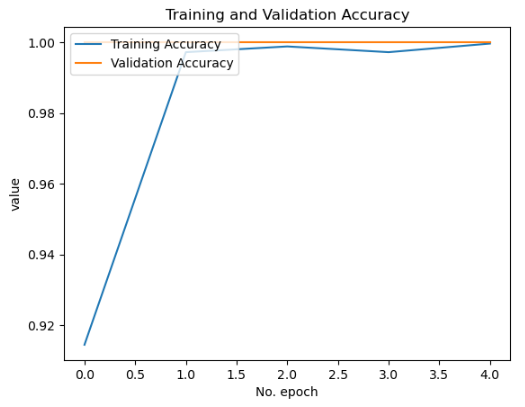
\includegraphics[width=0.64\linewidth]{../Gambar/akurasi.png}
  \caption{Grafik \emph{training} dan \emph{validation} akurasi}
  \label{fig:akurasi}
\end{figure}

Setelah proses \emph{training} selesai dan telah didapatkan model dengan akurasi yang tinggi atau sesuai \emph{threshold} dalam hal ini dapat dilihat pada grafik akurasi pada Gambar \ref{fig:akurasi}, maka selanjutnya masuk kepada proses evaluasi model. Evaluasi model menggunakan \emph{confusion matrix} dengan data testing citra sebanyak 100 pada masing-masing kelas. Hasil dari \emph{confusion matrix} didapatkan akurasi 100\%. Hasil evaluasi dengan \emph{confusion matrix} secara lengkap dapat dilihat pada Gambar \ref{fig:confusionmatrix}. Data pada kelas diam, kanan, maju, dan mundur mendapatkan nilai klasifikasi benar 100 sedangkan pada kelas kiri mendapatkan nilai klasifikasi benar 99. Model yang telah dievaluasi menggunakan \emph{confusion matrix} selanjutnya digunakan sebagai klasifikasi. Klasifikasi menghasilkan kode instruksi yang digunakan sebagai acuan dalam memberikan perintah kepada robot. Klasifikasi dilakukan dengan menggunakan model yang telah dibuat dan citra dataset baru. Citra dataset akan diolah sama dengan citra yang digunakan \emph{training} yaitu mulai dari menggambar \emph{hand landmark}, ekstraksi fitur, dan citra trnasformasi. Citra transformasi akan dikenali pose didalamnya dan hasil pengenalan citra tersebut diubah menjadi kode instruksi dan dikirim kepada robot. Adapun kode instruksi yang diatur sebagai perintah kepada robot dapat dilihat pada Tabel \ref{tab:kodeinstruksi}

\begin{figure}[H]
  \centering
  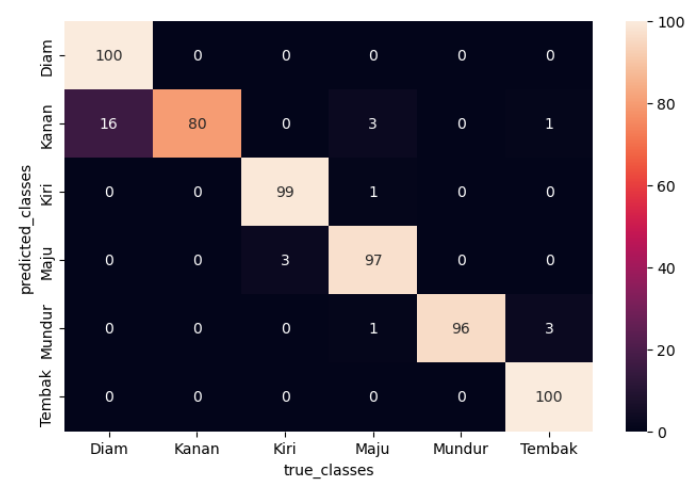
\includegraphics[width=0.8\linewidth]{../Gambar/confusionmatrix.png}
  \caption{Hasil \emph{Confusion Matrix}}
  \label{fig:confusionmatrix}
\end{figure}

\begin{table}[H]
  \centering
  \caption{Kode instruksi hasil klasifikasi}
  \label{tab:kodeinstruksi}
  \begin{tabular}{|c|c|}
  \hline
  Pose   & Kode Instruksi \\ \hline
  Diam   & n              \\ \hline
  Kanan  & r              \\ \hline
  Kiri   & l              \\ \hline
  Maju   & f              \\ \hline
  Mundur & b              \\ \hline
  Tangan tidak terdeteksi & n              \\ \hline
  \end{tabular}
\end{table}

\subsection{Kontrol Navigasi}
Proses kontrol navigasi diawali dengan perancangan komunikasiantara laptop dengan robot dan dilanjutkan perancangan pada robot. Komuniasi antara laptop dengan robot menggunakan \emph{web socket}. Robot dirancang dengan memiliki kemampuan untuk bergerak dan menembak.  Kebutuhan robot dengan adanya kemampuan bergerak dan menembak membutuhkan mikrokontroler untuk mengatur semua itu dan juga untuk koneksi secara \emph{wireless} dengan laptop. \emph{Mikrokontroller} yang digunakan yaitu "nodeMCU ESP8266" dengan alasan sudah memiliki modul \emph{WiFi} yang terpasang didalamnya dan juga memiliki kemampuan yang cukup untuk dapat mengontrol robot. Pergerakan robot dapat terjadi dikarenakan adanya sepasang roda yang dipasangkan pada robot. Untuk menggerakkan roda pada robot dibutuhkan motordc yang dipasangkan pada roda. Motordc yang digunakan berjumlah dua buah yang dipasangkan pada robot. Motordc dapat menggerakkan roda ketika dialiri oleh arus listrik. \emph{Mikrokontroller} tidak dapat secara langsung mengatur aliran listrik yang masuk kepada motordc, maka dari itu dibutuhkannya \emph{motor driver}. Arus listrik yang akan mengalir ke motor dc akan diatur oleh motor driver. Semakin kuat arus listrik yang mengalir ke motor dc maka akan semakin cepat perputaran roda yang mengakibatkan semakin cepat pergerakan dari robot. Secara schematic dapat dilihat pada Gambar \ref{fig:schematic}. Dari schematic yang telah dibuat dibuatlah robot yang dapat dilihat pada Gambar \ref{fig:hasilrobot}.
% Kemampuan menembak pada robot diatur dengan adanya sensor \emph{infrared}. Sensor \emph{infrared transmitter} diletakkan di depan robot sedangkan sensor \emph{infrared receiver} membutuhkan empat yang diletakkan disekeliling sisi robot. Sensor \emph{infrared transmitter} diletakkan di depan dengan tujuan saat menembak, arah tembakan robot ke depan searah dengan robot. Saat menembak robot terlebih dahulu dan kemudian mengaktifkan sensor \emph{infrared transmitter} sebagai simbol dari menembak. Saat menembak sensor \emph{infrared transmitter} akan mengirimkan pesan dalam bentuk \emph{hexadecimal} dan pada masing-masing robot akan memiliki nilai \emph{hexadecimal} yang berbeda. Sensor \emph{infrared receiver} di sambungkan secara pararel untuk ke empat sensornya dan dihubungkan kepada mikrokontroler. Sensor \emph{infrared receiver} diletakkan disekeliling dengan tujuan robot dapat tertembak dari segala arah. Saat sensor \emph{infrared receiver} menerima tembakan maka akan dicek terlebih dahulu pesan \emph{hexadecimal} yang diterima. Pesan yang diterima oleh sensor \emph{infrared receiver} dan sesuai dengan pesan \emph{hexadecimal} dari yang dikirim robot maka pesan terbesut dikirim kepada laptop melalu koneksi internet. 

\begin{figure}[H]
  \centering
  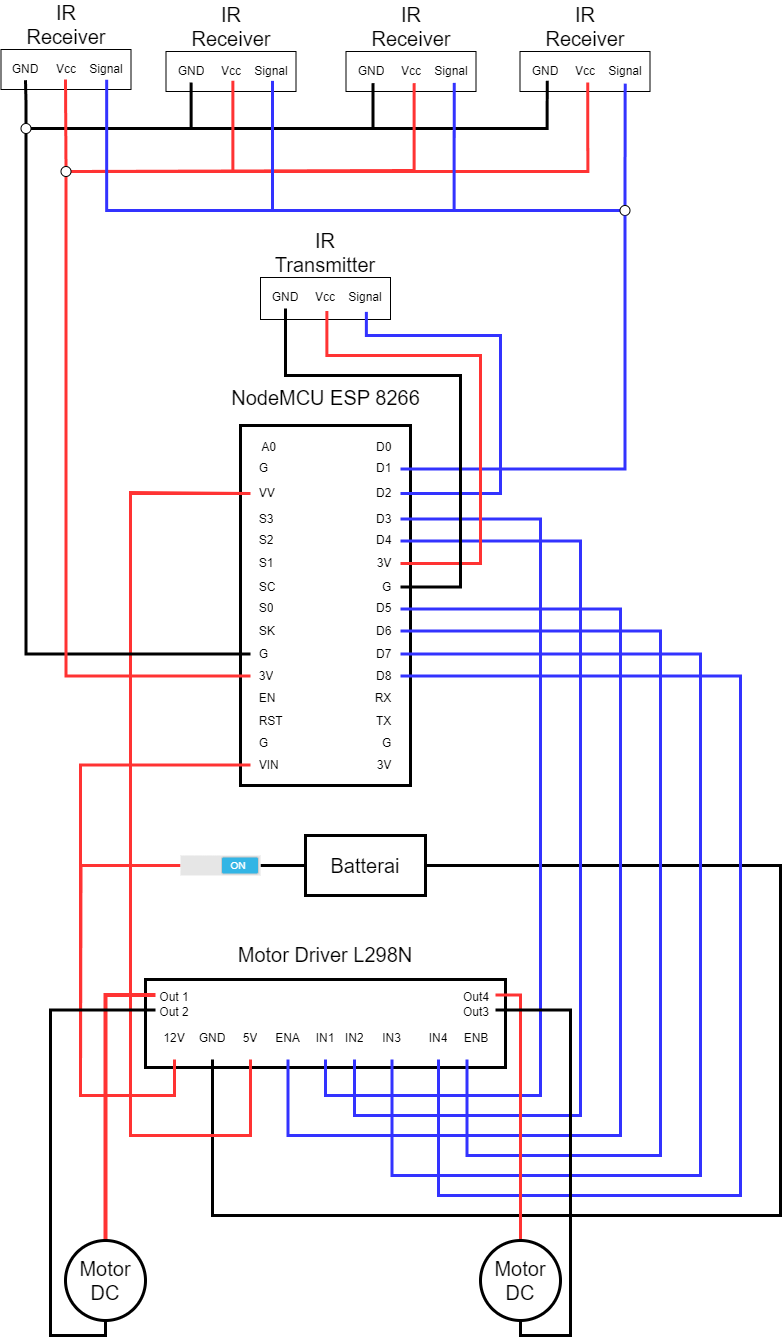
\includegraphics[width=0.6\linewidth]{../Gambar/schematic.png}
  \caption{\emph{Schematic} robot}
  \label{fig:schematic}
\end{figure}

\begin{figure}[H]
  \begin{subfigure}{0.8\textwidth}
    \centering
    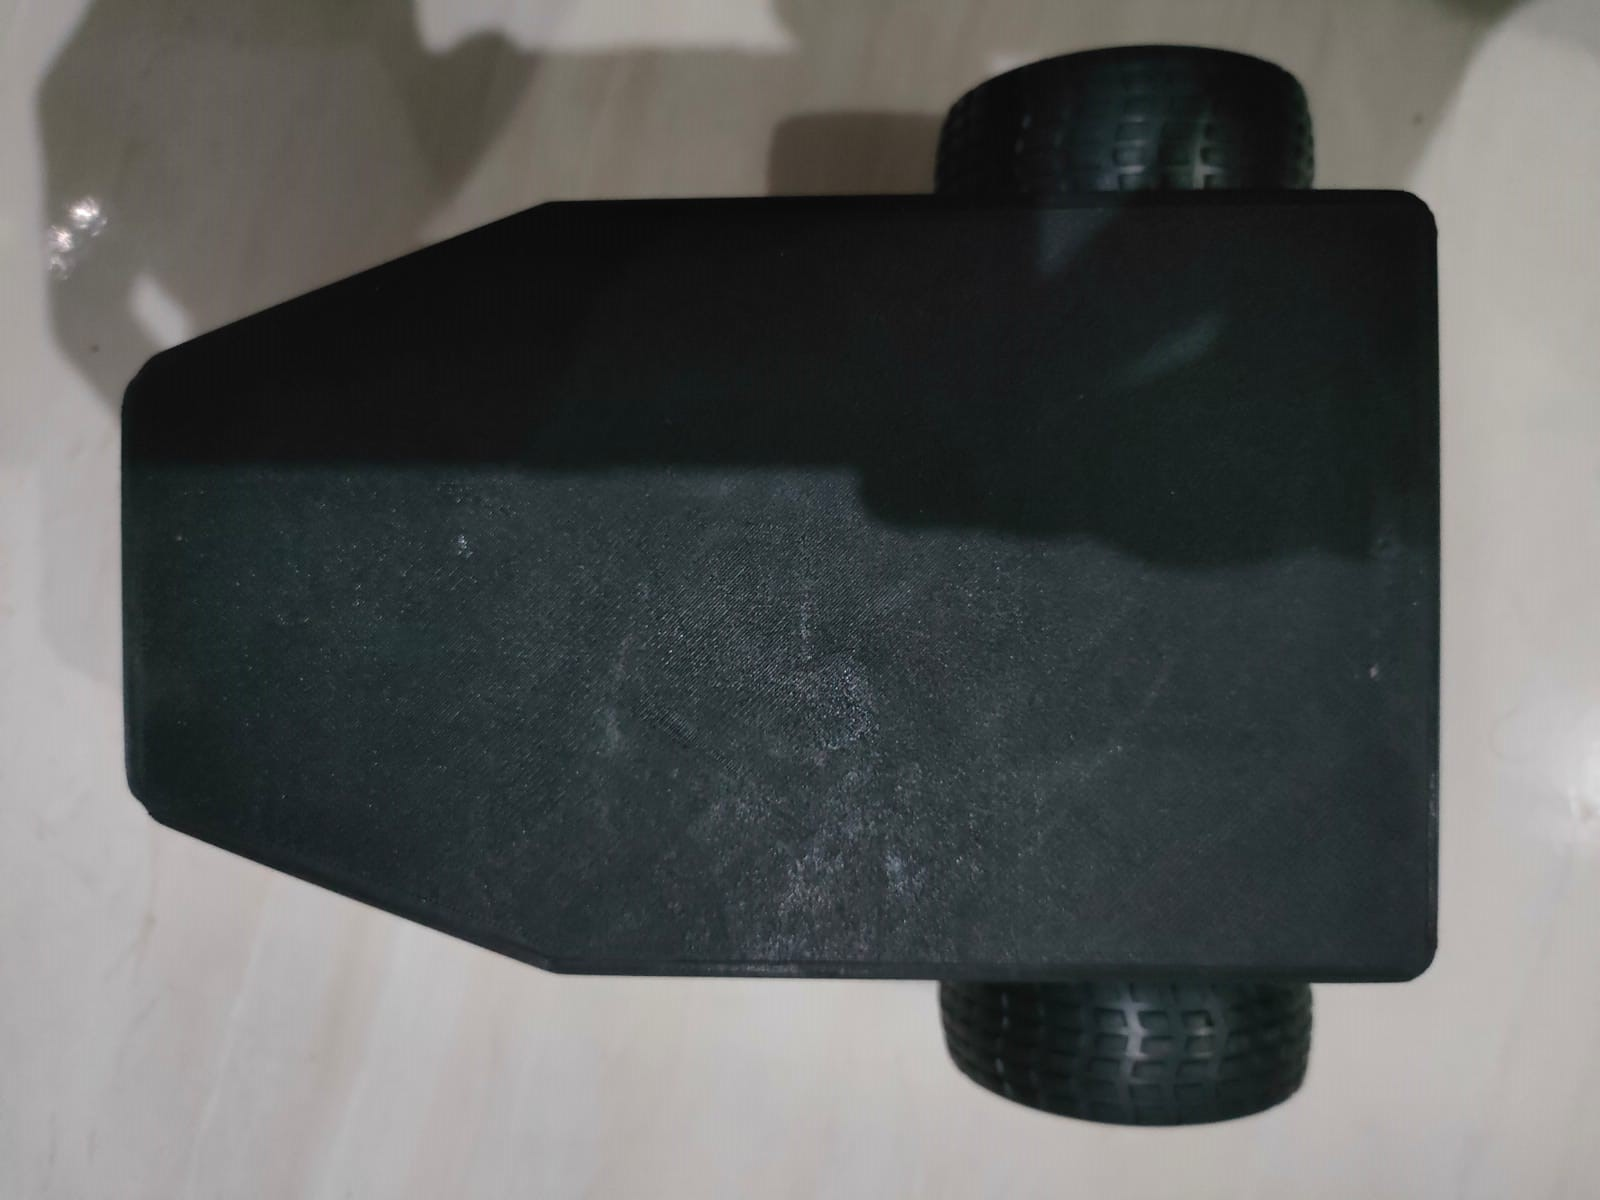
\includegraphics[width=\linewidth]{../Gambar/dengantutup.jpg}
    \caption{Dengan tutup}
    \label{fig:dengantutup}
  \end{subfigure}
  \begin{subfigure}{0.8\textwidth}
    \centering
    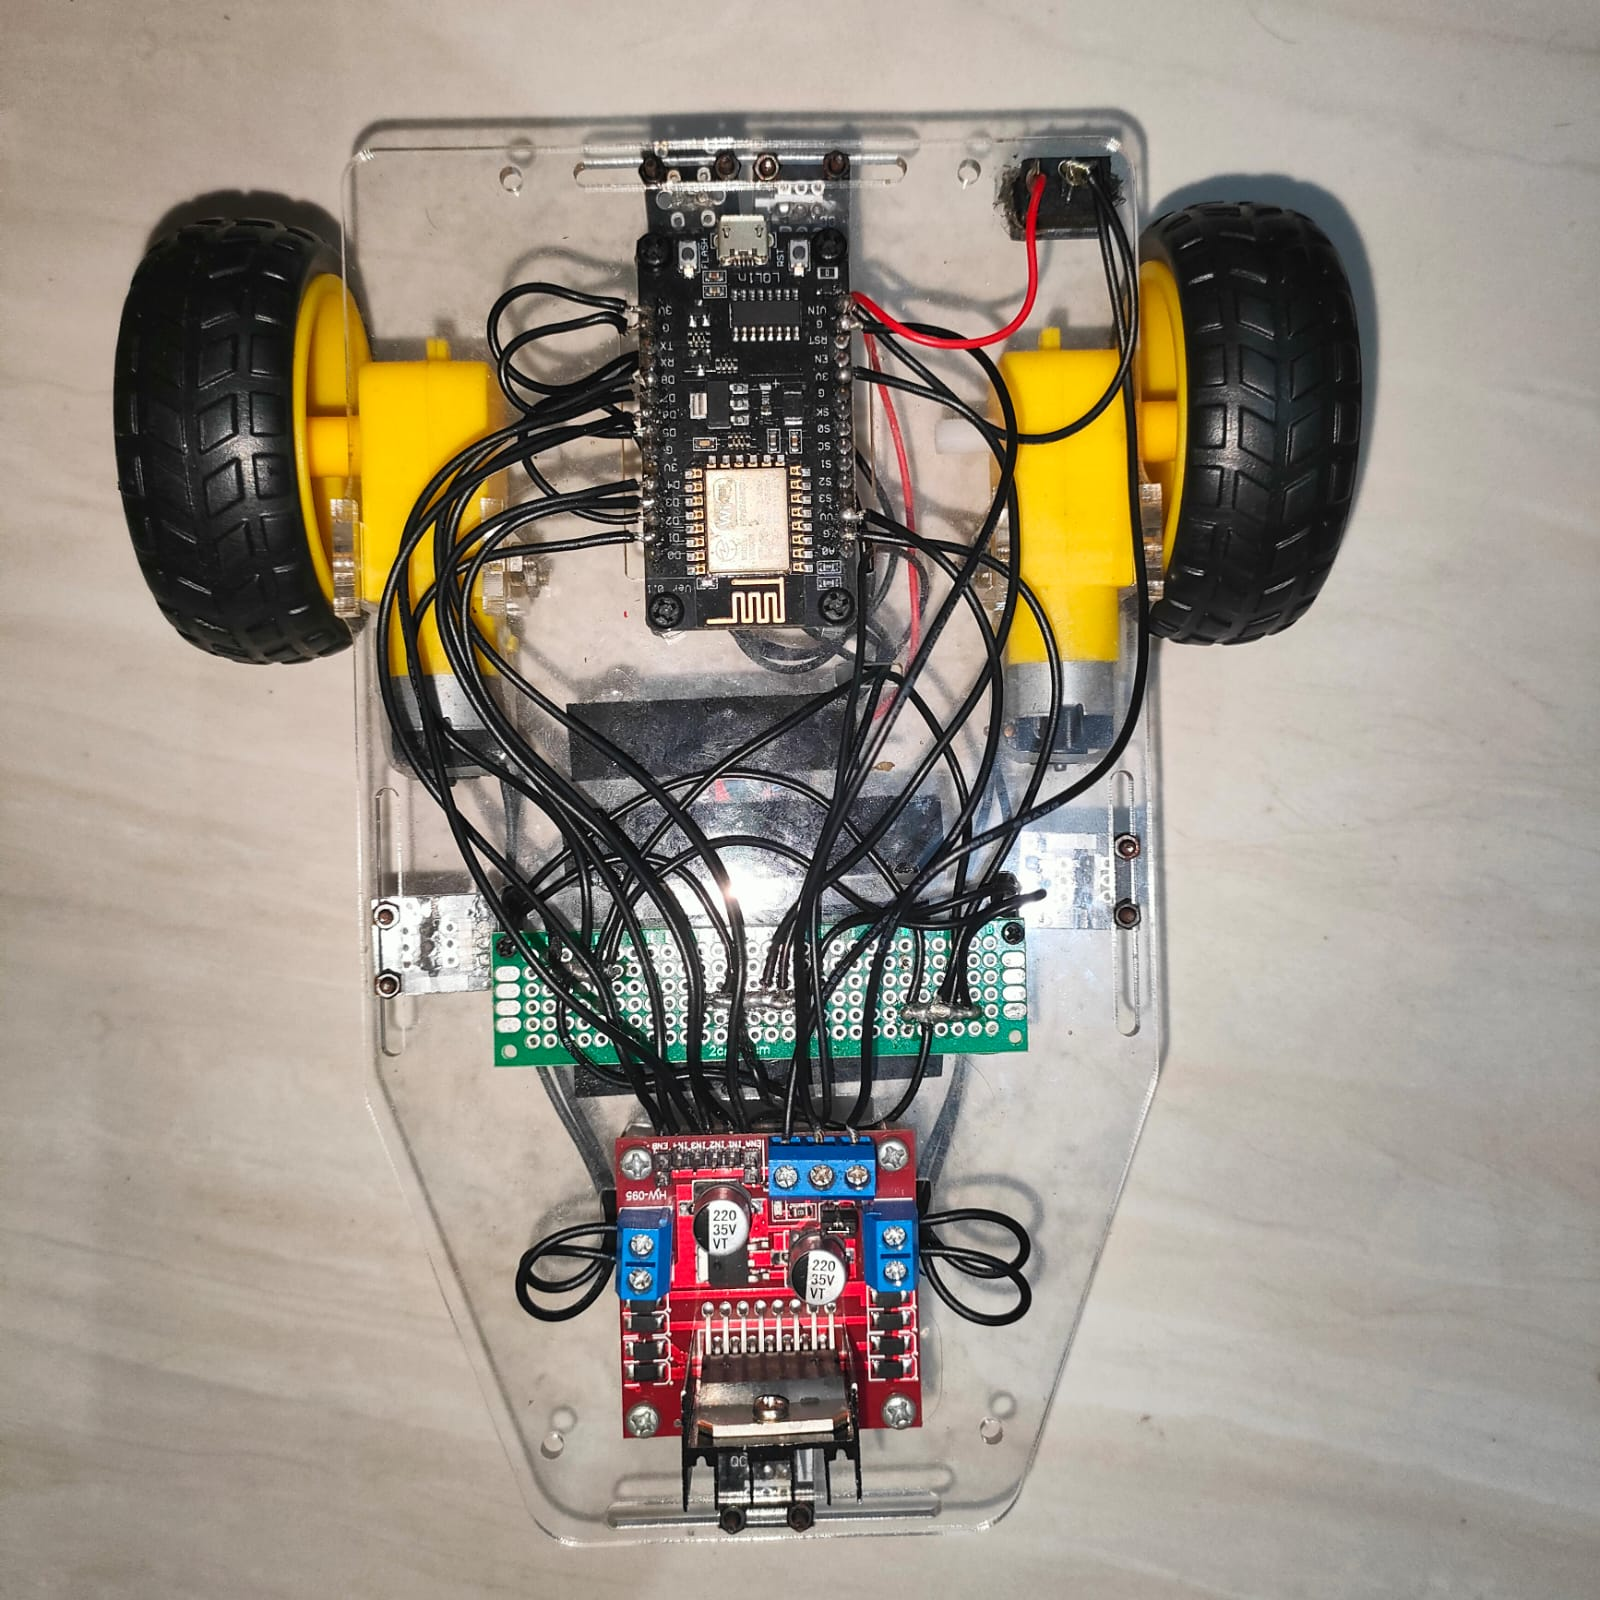
\includegraphics[width=\linewidth]{../Gambar/tanpatutup.jpg}
    \caption{Tanpa tutup}
    \label{fig:tanpatutup}
  \end{subfigure}
  \centering
  \caption{Hasil robot yang dirancang tampak dari atas}
  \label{fig:hasilrobot}
\end{figure}

\section{Skenario Pengujian}
Pada bab ini dilakukan beberapa skenario pengujian untuk mengetahui tingkat kesalahan dan kondisi ideal yang dapat digunakan sebagai kondisi untuk mengendalikan robot. Pengujian dilakukan untuk menarik kesimpulan secara keseluruhan serta membuka potensi pengembangan penelitian dimasa mendatang. Secara spesifik skenario pengujian yang dilakukan sebagi berikut.
\subsection{Pengujian Jarak Kamera terhadap Tangan}
\label{sub:jarak}
Pengujian ini menggunakan tangan peneliti yang digunakan pada pembuatan dataset dengan variasi jarak tangan terhadap kamera. Pengujian jarak dilakukan untuk mengetahui jarak ideal dari model. Jarak yang dimaksud merupakan jarak antara kamera dengan  kedua tangan. Ketinggian dari tangan sejajar dengan kamera serta telapak tangan menghadap kepada kamera dan berada tepat didepan kamera. Pengujian jarak dilakukan dengan cara mengambil 20 citra dari tiap kelas pada jarak tertentu. Jarak ini dimulai dari 40cm, 60cm, 80cm, 100cm, 120cm, dan 140cm antara tangan dengan kamera. Pengujian jarak dimulai dari jarak 40cm dikarenakan jika kurang dari 40cm maka tangan yang terdeteksi dapat melebihi area yang tertangkap oleh kamera. Pengujian dilakukan karena adanya perubahan ukuran dari tangan yang dipengaruhi oleh jarak kamera terhadap tangan. Hasil pengambilan citra dari jarak 40cm sampai 140cm dapat dilihat pada Gambar \ref{fig:jarakkeseluruhan}. 

\begin{figure}[H]
  \centering
  \begin{subfigure}{0.4\textwidth}
    \centering
    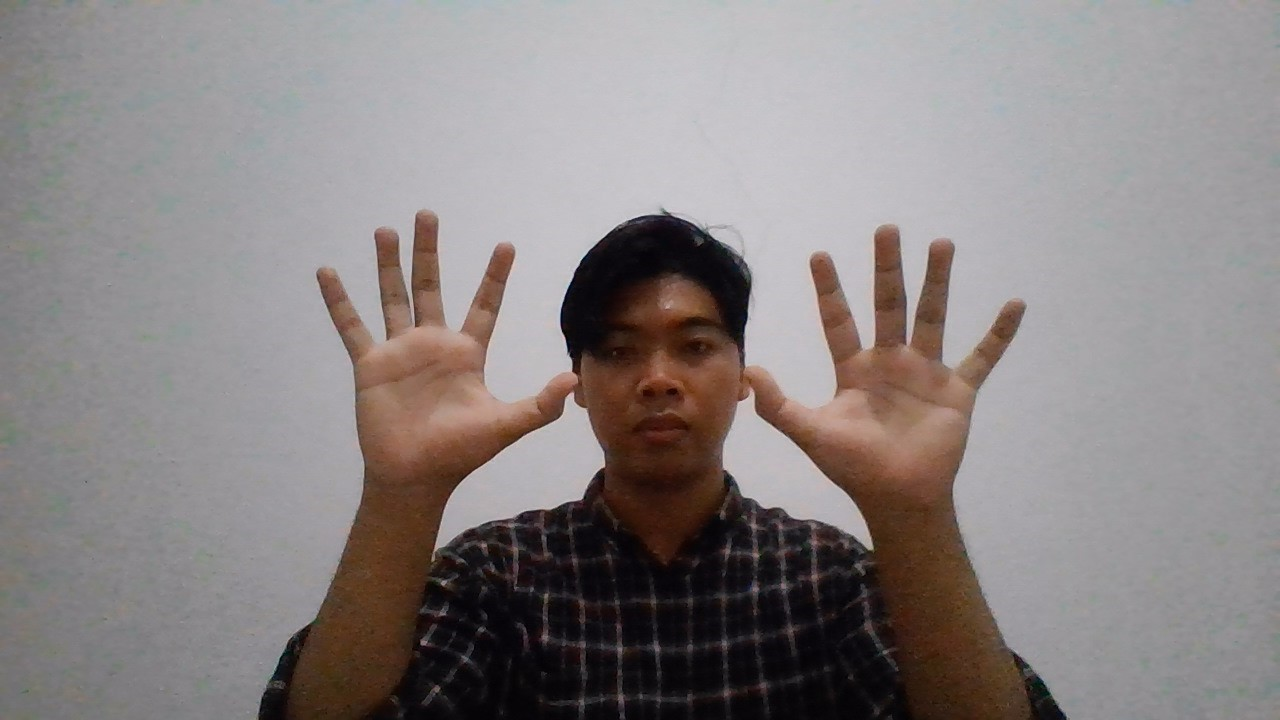
\includegraphics[width=\linewidth]{../Gambar/40cm.jpg}
    \caption{Jarak 40cm}
    \label{fig:jarak40cm}
  \end{subfigure}
  \begin{subfigure}{0.4\textwidth}
    \centering
    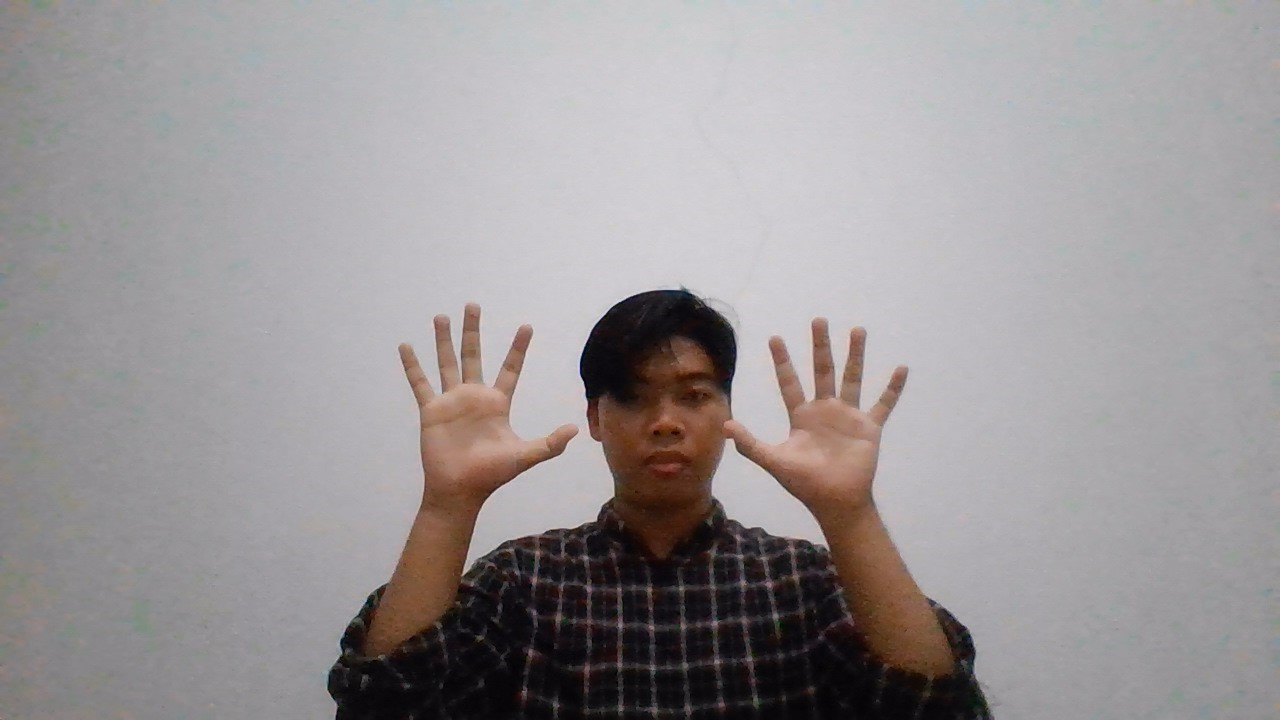
\includegraphics[width=\linewidth]{../Gambar/60cm.jpg}
    \caption{Jarak 60cm}
    \label{fig:jarak60cm}
  \end{subfigure}
  \begin{subfigure}{0.4\textwidth}
    \centering
    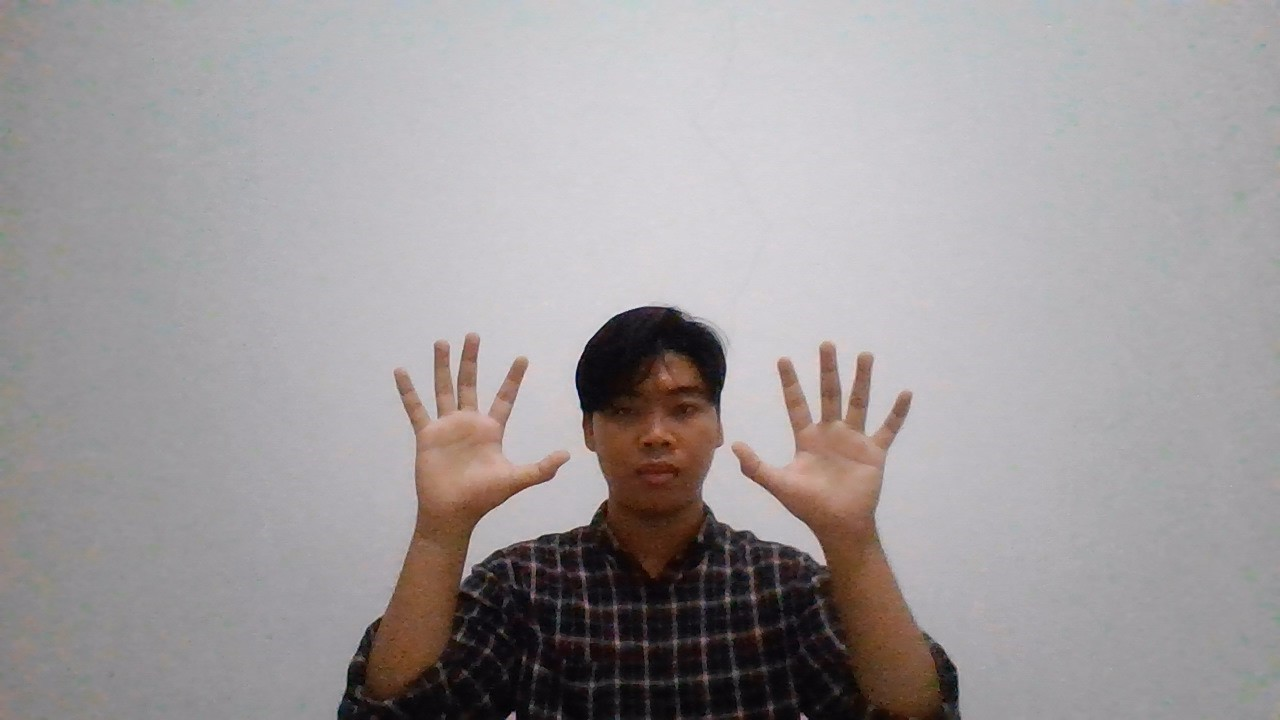
\includegraphics[width=\linewidth]{../Gambar/80cm.jpg}
    \caption{Jarak 80cm}
    \label{fig:jarak80cm}
  \end{subfigure}
  \begin{subfigure}{0.4\textwidth}
    \centering
    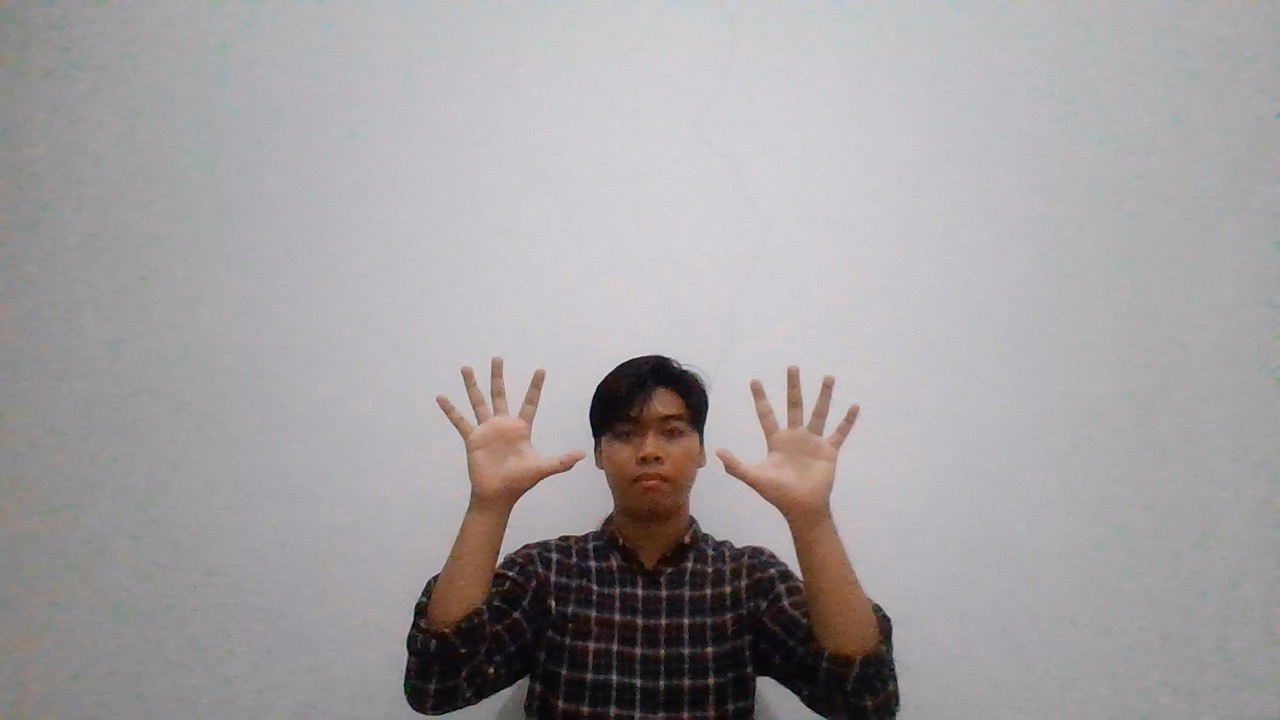
\includegraphics[width=\linewidth]{../Gambar/100cm.jpg}
    \caption{Jarak 100cm}
    \label{fig:jarak100cm}
  \end{subfigure}
  % \begin{subfigure}{0.4\textwidth}
  %   \centering
  %   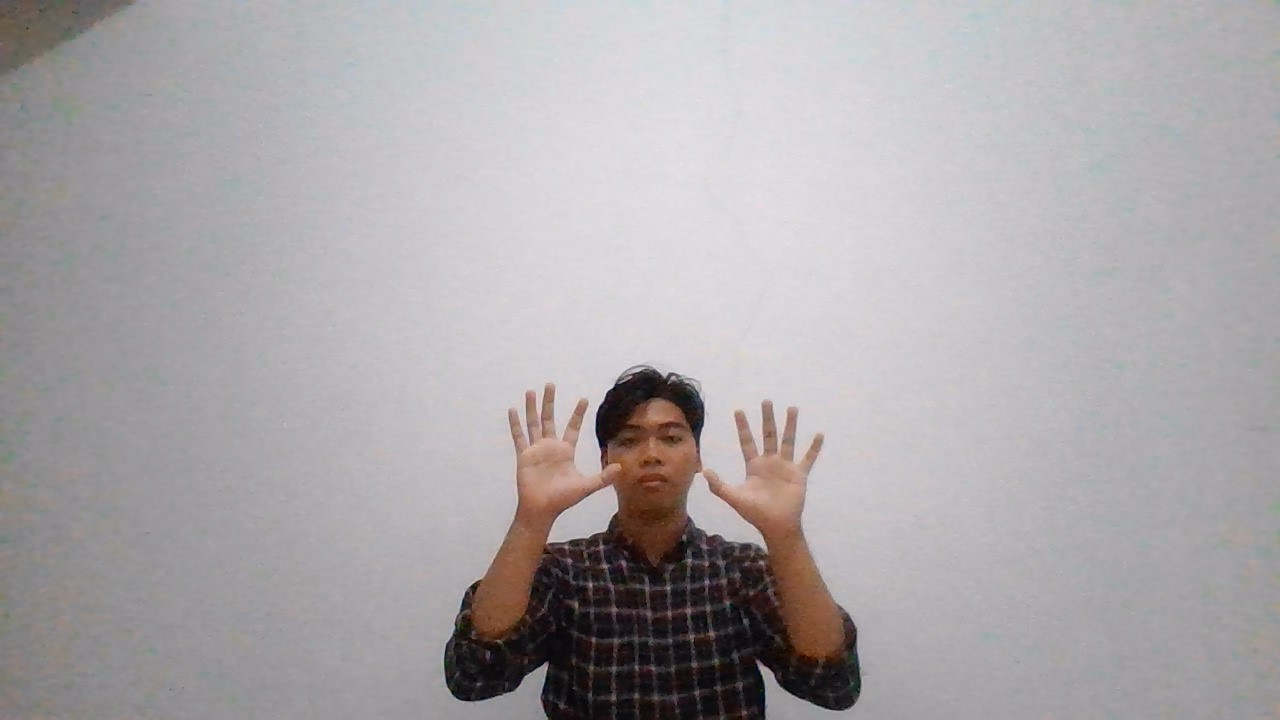
\includegraphics[width=\linewidth]{../Gambar/120cm.jpg}
  %   \caption{Jarak 120cm}
  %   \label{fig:jarak120cm}
  % \end{subfigure}
  % \begin{subfigure}{0.4\textwidth}
  %   \centering
  %   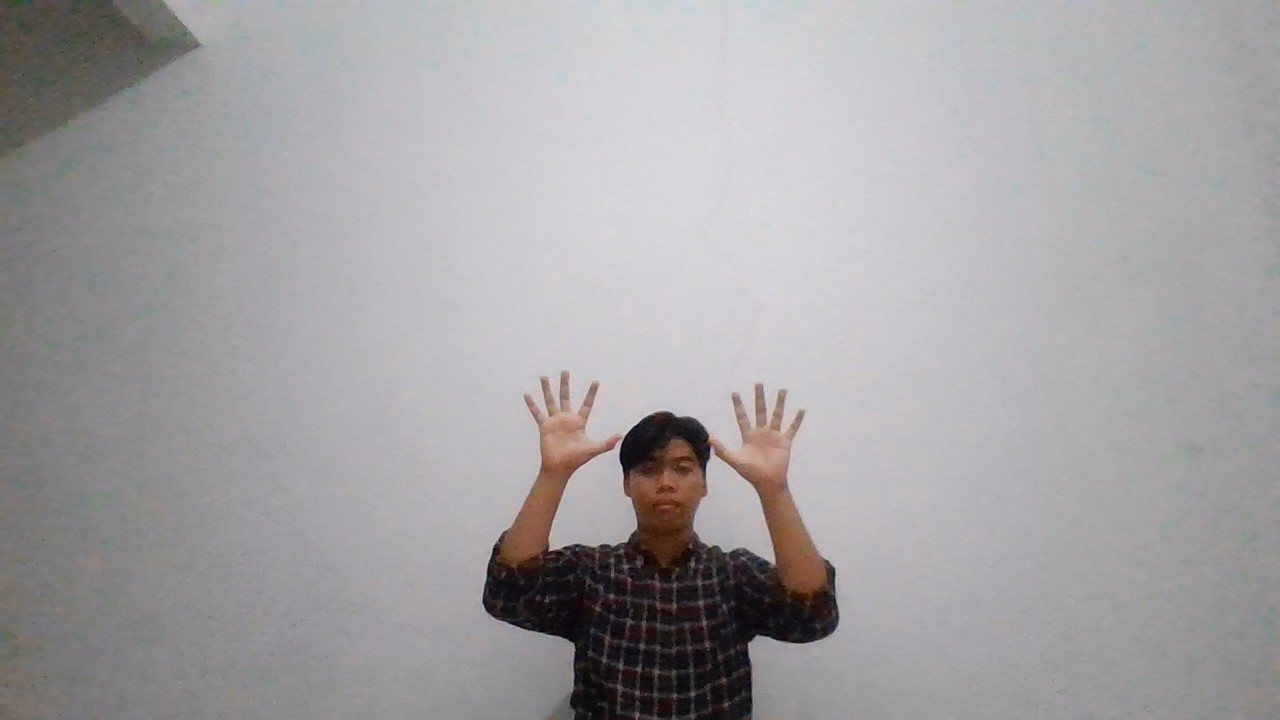
\includegraphics[width=\linewidth]{../Gambar/140cm.jpg}
  %   \caption{Jarak 140cm}
  %   \label{fig:jarak140cm}
  % \end{subfigure}
  % \caption{Citra Pengujian Variasi Jarak}
  % \label{fig:jarakkeseluruhan}
\end{figure}

\begin{figure}[H]
%   \begin{subfigure}{0.4\textwidth}
%     \centering
%     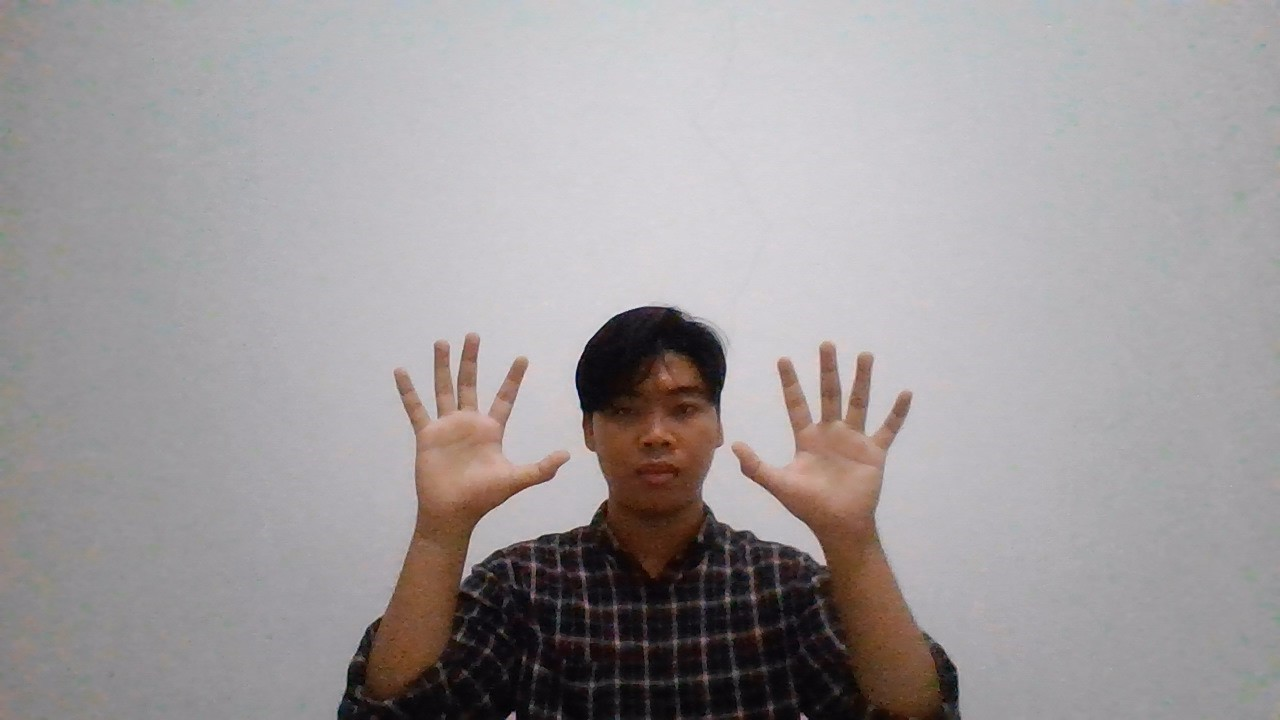
\includegraphics[width=\linewidth]{../Gambar/80cm.jpg}
%     \caption{Jarak 80cm}
%     \label{fig:jarak80cm}
%   \end{subfigure}
%   \begin{subfigure}{0.4\textwidth}
%     \centering
%     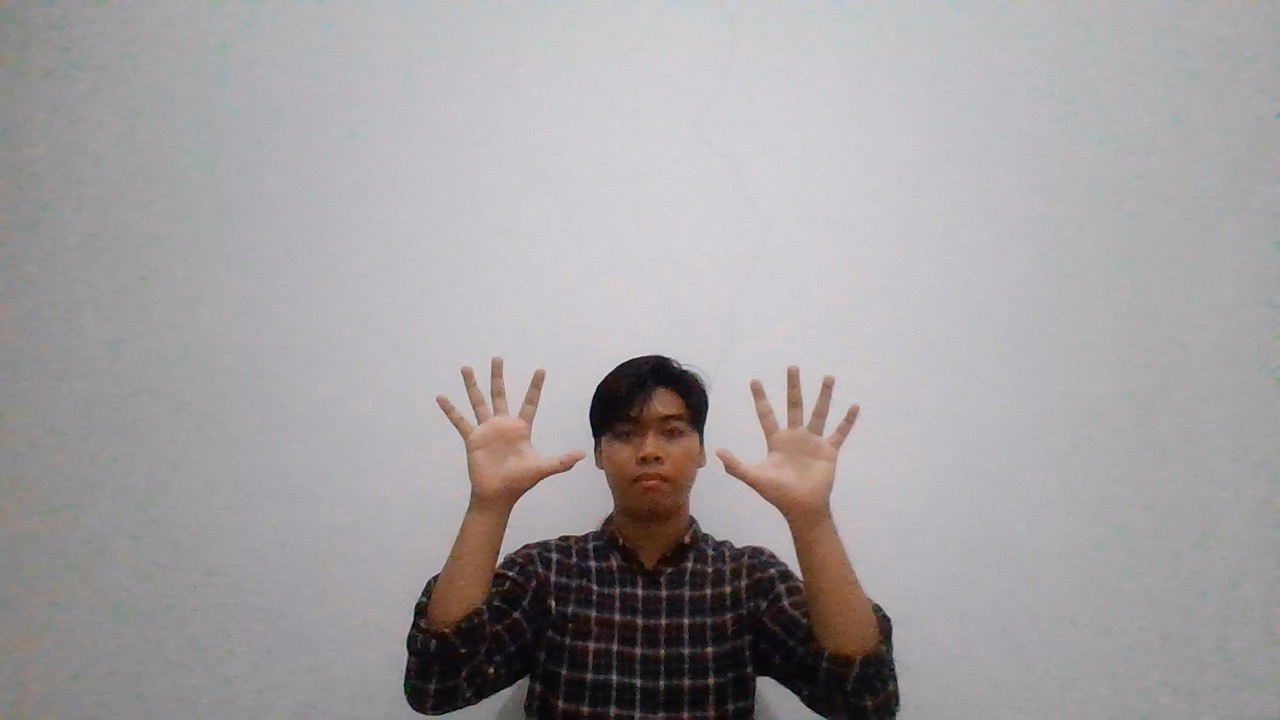
\includegraphics[width=\linewidth]{../Gambar/100cm.jpg}
%     \caption{Jarak 100cm}
%     \label{fig:jarak100cm}
%   \end{subfigure}
  \begin{subfigure}{0.4\textwidth}
    \centering
    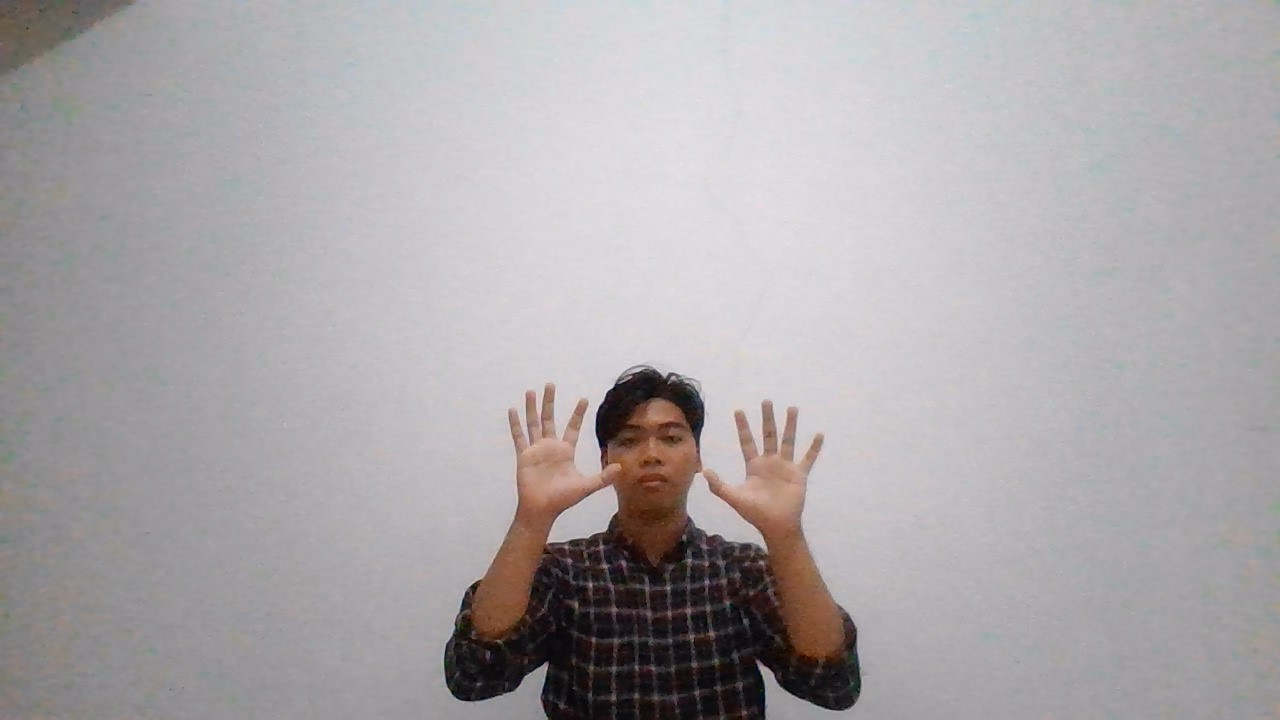
\includegraphics[width=\linewidth]{../Gambar/120cm.jpg}
    \caption{Jarak 120cm}
    \label{fig:jarak120cm}
  \end{subfigure}
  \begin{subfigure}{0.4\textwidth}
    \centering
    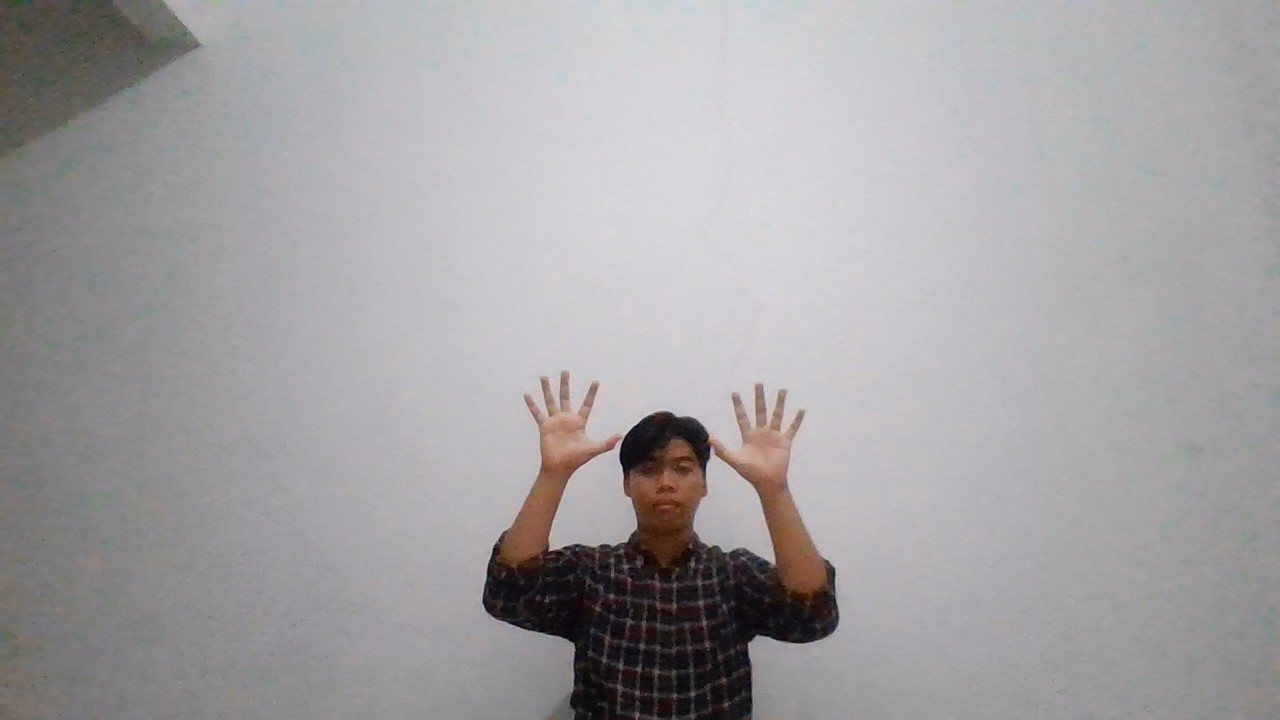
\includegraphics[width=\linewidth]{../Gambar/140cm.jpg}
    \caption{Jarak 140cm}
    \label{fig:jarak140cm}
  \end{subfigure}
  \centering
  \caption{Citra Pengujian Variasi Jarak}
  \label{fig:jarakkeseluruhan}
\end{figure}

Setelah 100 citra telah diambil dilakukan pengujian terhadap model yang telah dibuat. Evaluasi terhadap model dilakukan menggunakan \emph{confusion matrix} dan didapatkan hasil estimasi pose tiap kelasnya. Hasil estimasi pose tiap kelas pada variasi jarak dari 40cm sampai 140cm dapat di lihat pada Gambar \ref{fig:confusionmatrixjarak}. Pada jarak 40cm didapatkan data klasifikasi benar pada kelas Diam, Maju, dan Mundur adalah 20. Pada kelas Kanan mendapatkan 17 data klasifikasi benar dan Kiri mendapatkan 19 data klasifikasi benar. Pada kelas Kanan dan Kiri terdapat kesalahan klasifikasi menjadi kelas Diam. Pada jarak 60cm hasil \emph{confusion matrix} mendapatkan 20 data klasifikasi benar pada kelas Kanan, Kiri, Maju, dan Mundur. Pada kelas Diam mendapatkan data prediski benar sebesar 19. Pada jarak 80cm dan 100cm mendapatkan data klasifikasi benar dengan nilai 20 pada semua kelas. Pada jarak 120cm pada kelas Diam dan Maju mendapatkan nilai 20 untuk data klasifikasi benar dan pada kelas Kanan mendapatkan nilai 18 data klasifikasi benar. Pada kelas Kiri mendapatkan nilai 16 untuk data klasifikasi benar dan niali 17 untuk kelas Mundur. Pada jarak 140cm didapatkan nilai 20 untuk data klasifikasi benar pada kelas Diam dan Maju. Pada kelas Kanan mendapatkan nilai 19 data klasifikasi benar dan pada kelas Kiri mendapatkan nilai 2 pada data klasifikasi benar. Pada jarak 140cm kelas Mundur mendapatkan niali 14 data klasifikasi benar. Dari hasil \emph{confusion matrix} dapat diketahui nilai akurasi dari tiap variasi pengujian. Hasil perhitungan nilai akurasi pada tiap variasi dapat dilihat pada Tabel \ref{tab:hasiljarak}. Dari hasil pengujian didapatkan nilai akurasi tertinggi pada jarak 80 cm dan 100cm yaitu dengan nilai akurasi 100\% dengan jumlah data percobaan 100 dan data yang terbaca benar juga 100. Pada jarak 40cm didapatkan nilai akurasi sebesar 96\% dengan jumlah data percobaan 100 dan data yang terbaca benar sebanyak 96. Pada jarak 60cm didapatkan nilai akurasi yaitu 99\% dengan jumlah data percobaan 100 dan data yang berhasil dibaca dengan benar sebanyak 99. Pada jarak 120cm didaptakn nilai akurasi 91\% dengan jumlah data percobaan 100 data dan data yang berhasil dibaca dengan benar sebanyak 91 data. Pada jarak 140cm nilai akurasi menurun menjadi 75\% dengan jumlah data percobaan sebanyak 100 data dan data yang terbaca benar sebanyak 75 data. Dari nilai akurasi ini didapatkan jarak ideal untuk dilakukannya klasifikasi menggunakan model yang telah dibuat berada pada jarak 40cm sampai 120cm pada tangan peneliti yang digunakan sebagai dataset. Dari hasil \emph{confusion matrix} data yang terbaca salah pada jarak 140cm di kelas Kiri terbaca mejadi kelas Diam. Dari hasil confusion matrix didapatkan analisa bahawa kelas yang cenderung dikenali adalah kelas Maju dan Diam dikarenakan terdapat perbuhan pose yang signifikan antara kedua kelas ini. Pada kelas Kiri dan Kanan memiliki kecenderungan data dibaca sebagai Maju atau Diam dikarenakan kelas Kiri dan Kanan dibuat dari campuran pose Diam dan Maju.

\begin{figure}[H]
  \begin{subfigure}{0.4\textwidth}
    \centering
    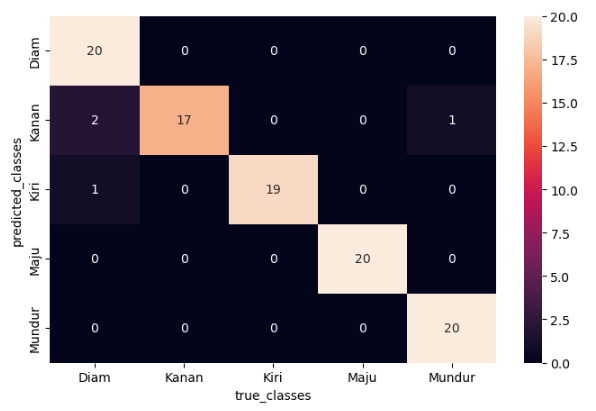
\includegraphics[width=\linewidth]{../Gambar/cm40.png}
    \caption{Jarak 40cm}
    \label{fig:cm40}
  \end{subfigure}
  \begin{subfigure}{0.4\textwidth}
    \centering
    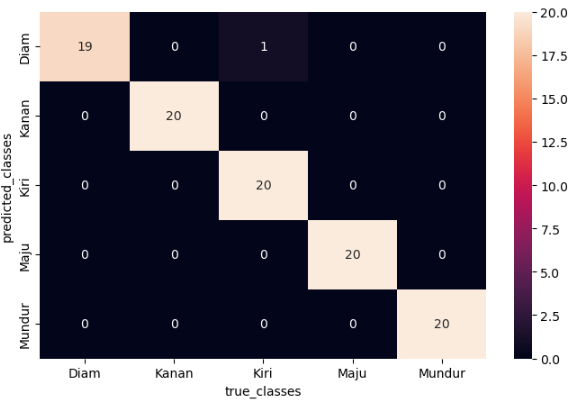
\includegraphics[width=\linewidth]{../Gambar/cm60.png}
    \caption{Jarak 60cm}
    \label{fig:cm60}
  \end{subfigure}
  \begin{subfigure}{0.4\textwidth}
    \centering
    \includegraphics[width=\linewidth]{../Gambar/cm80.png}
    \caption{Jarak 80cm}
    \label{fig:cm80}
  \end{subfigure}
  \begin{subfigure}{0.4\textwidth}
    \centering
    \includegraphics[width=\linewidth]{../Gambar/cm100.png}
    \caption{Jarak 100cm}
    \label{fig:cm100}
  \end{subfigure}
  \begin{subfigure}{0.4\textwidth}
    \centering
    \includegraphics[width=\linewidth]{../Gambar/cm120.png}
    \caption{Jarak 120cm}
    \label{fig:cm120}
  \end{subfigure}
  \begin{subfigure}{0.4\textwidth}
    \centering
    \includegraphics[width=\linewidth]{../Gambar/cm140.png}
    \caption{Jarak 140cm}
    \label{fig:cm140}
  \end{subfigure}
  \centering
  \caption{Hasil \emph{Confusion Matrix} Berdasarkan  Varias Jarak}
  \label{fig:confusionmatrixjarak}
\end{figure}

\begin{table}[H]
  \centering
  \caption{Hasil Akurasi Berdasarkan Variasi Jarak}
  \label{tab:hasiljarak}
  \begin{tabular}{|c|c|c|c|c|}
    \hline
    Jarak (cm) & Jumlah Percobaan & Terbaca Benar & \multicolumn{1}{l|}{Terbaca Salah} & \multicolumn{1}{l|}{Akurasi} \\ \hline
    40         & 100              & 96           & 4                                  & 94\%                        \\ \hline
    60         & 100              & 99           & 1                                  & 99\%                         \\ \hline
    80         & 100              & 100           & 0                                  & 100\%                         \\ \hline
    100        & 100              & 100           & 0                                  & 100\%                         \\ \hline
    120        & 100              & 91            & 9                                 & 91\%                         \\ \hline
    140        & 100              & 75            & 25                                 & 75\%                         \\ \hline
    \end{tabular}
\end{table}


\subsection{Pengujian Pengaruh Posisi dan Hadap Tangan terhadap Kamera}
\label{sub:posisidansudut}
Pengujian posisi dan hadap tangan terhadap kamera dilakukan menggunakan tangan peniliti dengan jarak uji 80cm dari kamera. Terdapat empat posisi yang akan diujikan yaitu pertama tepat didepan kamera dan memiliki ketinggian yang sama dengan kamera dengan variasi hadap tangan yang terhadap kamera yaitu serong ke kanan, serong ke kiri, serong ke bawah, dan serong ke atas. Posisi kedua diujikan dengan tangan untuk pengujian bergeser 40cm ke kiri kamera dengan menggunakan variasi hadap tangan yaitu menghadap ke arah kamera dan menghadap ke depan. Posisi ketiga diujikan dengan tangan untuk pengujian bergeser 40cm ke kanan kamera dengan variasi hadap yang digunakan yaitu menghadap ke arah kamera dan menghadap ke depan. Posisi ke empat tangan yang digunakan untuk pengujian bergeser 40cm ke atas kamera dengan variasi hadap menghadap ke arah kamera dan menghadap ke depan. Pengujian ini dilakukan untuk mengatahui kemampuan model terhadap variasi posisi tangan dan hadap yang tidak tepat didepan kamera, karena dataset yang digunakan tangan tepat berada didepan kamera.

\begin{enumerate}
  \item Posisi Tengah \par
  Pada posisi ini dilakukan empat pengujian dengan variasi hadap yaitu serong ke kanan, serong ke kiri, serong ke atas, dan serong ke bawah. Skenario pengujian dapat dilihat pada Gambar \ref{fig:posisitengah}. Setelah 100 citra telah diambil dilakukan pengujian terhadap model yang telah dibuat. Evaluasi terhadap model dilakukan menggunakan \emph{confusion matrix} dan didapatkan hasil estimasi pose tiap kelas. Hasil confusion matrix tiap variasi hadap dapat dilihat pada Gambar \ref{fig:cmtengah}. Pada serong ke kanan didapatkan data klasifikasi benar bernilai 20 pada kelas Kanan, Maju, dan Mundur. Pada kelas Diam didapatkan data klasifikasi benar sebesar sebelas dan sembilan data klasifikasi salah terklasifikasi pada kelas Kanan. Pada kelas Kiri didapatkan 16 data klasifikasi benar dan empat data klasifikasi salah terklasifikasi menjadi kelas Maju. Pada serong ke kiri didapatkan data klasifikasi benar sebanyak 20 data pada kelas Diam dan Kanan. Pada kelas Kiri didapatkan data klasifikasi benar sebanyak 17 data dan klasifikasi salah sebanyak tiga data yang terklasifikasi menjadi kelas Mundur. Pada kelas Maju mendapatkan data klasifikasi benar sebanyak 19 data dengan satu data terklasifikasi menjadi kelas Kanan. Pada kelas Mundur mendapatkan data klasifikasi benar sebnyak 18 data dan dua data lainnya terklasifikasi menjadi kelas Diam. Pada serong ke atas didapatkan data klasifikasi benar sebanyak 20 data pada kelas Kiri, Maju, dan Mundur. Pada kelas Diam didapatkan data klasifikasi benar sebnayak 17 data dan tiga data terklasifikasi salah pada kelas Kanan. kelas Kanan mendapatkan data klasifikasi benar sebanyak satu data dan data terklasifikasi Maju sebanyak 19 data. Pada serong ke bawah didapatkan data klasifikasi benar sebanyak 20 data pada kelas Diam, Kanan, dan Mundur. Kelas Kiri mendapatkan data klasifikasi benar sebanyak satu data dan data terklasifikasi sebagai kelas Diam sebanyak 18 data dan kelas Kiri sebanyak satu data. Kelas Maju mendapatkan data klasifikasi benar sebanyak 18 data dan terklasifikasi kelas Kanan sebanyak dua data.

  \begin{figure}[H]
    \centering
    \begin{subfigure}{0.4\textwidth}
      \centering
      \includegraphics[width=\linewidth]{../Gambar/Tengahserongkanan.jpg}
      \caption{Serong Ke Kanan}
      \label{fig:serongkanan}
    \end{subfigure}
    \begin{subfigure}{0.4\textwidth}
      \centering
      \includegraphics[width=\linewidth]{../Gambar/Tengahserongkiri.jpg}
      \caption{Serong Ke Kiri}
      \label{fig:serongkiri}
    \end{subfigure}
    \begin{subfigure}{0.4\textwidth}
      \centering
      \includegraphics[width=\linewidth]{../Gambar/Tengahserongatas.jpg}
      \caption{Serong Ke Atas}
      \label{fig:serongatas}
    \end{subfigure}
    \begin{subfigure}{0.4\textwidth}
      \centering
      \includegraphics[width=\linewidth]{../Gambar/Tengahserongbawah.jpg}
      \caption{Serong Ke Bawah}
      \label{fig:serongbawah}
    \end{subfigure}
    \centering
    \caption{Skenario Pengujian Hadap Tangan Pada Posisi Tengah}
    \label{fig:posisitengah}
  \end{figure}

  \begin{figure}[H]
    \centering
    \begin{subfigure}{0.4\textwidth}
      \centering
      \includegraphics[width=\linewidth]{../Gambar/cmtengahkanan.png}
      \caption{Serong Ke Kanan}
      \label{fig:cmtengahkanan}
    \end{subfigure}
    \begin{subfigure}{0.4\textwidth}
      \centering
      \includegraphics[width=\linewidth]{../Gambar/cmtengahkiri.png}
      \caption{Serong Ke Kiri}
      \label{fig:cmtengahkiri}
    \end{subfigure}
    \begin{subfigure}{0.4\textwidth}
      \centering
      \includegraphics[width=\linewidth]{../Gambar/cmtengahatas.png}
      \caption{Serong Ke Atas}
      \label{fig:cmtengahatas}
    \end{subfigure}
    \begin{subfigure}{0.4\textwidth}
      \centering
      \includegraphics[width=\linewidth]{../Gambar/cmtengahbawah.png}
      \caption{Serong Ke Bawah}
      \label{fig:cmtengahbawah}
    \end{subfigure}
    \centering
    \caption{\emph{Confusion Matrix} Pengujian Hadap Tangan Pada Posisi Tengah}
    \label{fig:cmtengah}
  \end{figure}

  \begin{table}[H]
    \centering
    \caption{Hasil Akurasi Pengujian Hadap Tangan Pada Posisi Tengah}
    \label{tab:hasilposisitengah}
    \begin{tabular}{|c|c|c|c|c|}
      \hline
      Hadap Tangan & Jumlah Percobaan & Terbaca Benar & \multicolumn{1}{l|}{Terbaca Salah} & \multicolumn{1}{l|}{Akurasi} \\ \hline
      Serong Ke Kanan         & 100              & 87           & 13                                  & 87\%                        \\ \hline
      Serong Ke Kiri         & 100              & 94           & 6                                  & 94\%                         \\ \hline
      Serong Ke Atas         & 100              & 78           & 22                                  & 78\%                         \\ \hline
      Serong Ke Bawah        & 100              & 79           & 21                                  & 79\%                         \\ \hline
      \end{tabular}
  \end{table}

  Dari hasil \emph{confusion matrix} dapat diketahui nilai akurasi dari tiap variasi pengujian. Hasil perhitungan nilai akurasi pada tiap variasi dapat dilihat pada Tabel \ref{tab:hasilposisitengah}. Pada serong ke kanan didapatkan dataterbaca benar sebanyak 87 data dan data terbaca salah sebanyak 13 data, dengan nilai akurasi sebesar 87\%. Pada serong ke kiri didapatkan data terbaca benar sebanyak 94 data dan enam data terbaca salah, maka dari itu didapatkan niali akurasi sebesar 94\%. Pada serong ke atas didapatkan data terbaca benar sebanyak 78 data dan 22 data terbaca salah, maka dari itu didapatkan nilai akurasi sebesar 78\%. Pada serong ke bawah didapatkan data terbaca benar sebanyak 79 data dan 21 data terbaca sala, maka dari itu nilai akurasi didapatkan sebesar 79\%. Dari confusion matrix dan akurasi yang didapatkan bahwa model dapat mengklasifikasi data dengan posisi serong dengan catatan bahwa kelima jari tidak terutup dengan jari lainnya dan serong ke kiri mendapatkan nilai akurasi tertinggi sebanyak 94\%.

  \item Posisi Kanan
  
  Pada posisi ini dilakukan dua pengujian dengan variasi hadap tangan terhadap kamera yaitu menghadap kamera dan hadap ke depan. Skenario pengujian dapat dilihat pada Gambar \ref{fig:posisikanan}. Setelah citra telah diambil dilakukan pengujian terhadap model yang telah dibuat. Evaluasi terhadap model dilakukan menggunakan confusion matrix dan didapatkan jasil estimasi pose tiap kelas. Hasil confusion matrix tiap variasi dapat dilihat pada Gambar \ref{fig:cmkanan}. Pada hadap ke kamera didapatkan data klasifikasi benar sebanyak 20 data pada kelas Diam, Kiri, dan Maju. Pada kelas Kanan dan Mundur didapatkan 19 data klasifikasi benar dengan satu data terbaca Maju pada kelas Kanan dan satu data terbaca kelas Diam pada kelas Mundur. Pada hadap lurus didapatkan data klasifikasi benar sebanyak 20 data pada kelas Diam, Kanan, Kiri, dan Maju. Pada kelas mundur didapatkan data klasifikasi benar sebanyak 16 data dengan data terbaca salah sebanyak empat data dengan rincian tiga data pada kelas Diam dan satu data terklasifikasi sebagai kelas Kiri.

  \begin{figure}[H]
    \centering
    \begin{subfigure}{0.7\textwidth}
      \centering
      \includegraphics[width=\linewidth]{../Gambar/KananHadapKamera.jpg}
      \caption{Hadap Ke Kamera}
      \label{fig:kananhadapkamera}
    \end{subfigure}
    \begin{subfigure}{0.7\textwidth}
      \centering
      \includegraphics[width=\linewidth]{../Gambar/KananHadapLurus.jpg}
      \caption{Hadap Ke Depan}
      \label{fig:kananhadaplurus}
    \end{subfigure}
    \centering
    \caption{Skenario Pengujian Hadap Tangan Pada Posisi Kanan}
    \label{fig:posisikanan}
  \end{figure}

  \begin{figure}[H]
    \centering
    \begin{subfigure}{0.7\textwidth}
      \centering
      \includegraphics[width=\linewidth]{../Gambar/cmkananhadapkamera.png}
      \caption{Hadap Ke Kamera}
      \label{fig:cmkanankamera}
    \end{subfigure}
    \begin{subfigure}{0.7\textwidth}
      \centering
      \includegraphics[width=\linewidth]{../Gambar/cmkananhadaplurus.png}
      \caption{Hadap Ke Depan}
      \label{fig:cmkananlurus}
    \end{subfigure}
    \centering
    \caption{\emph{Confusion Matrix} Pengujian Hdap Tangan pada Posisi Kanan}
    \label{fig:cmkanan}
  \end{figure}

  \begin{table}[H]
    \centering
    \caption{Hasil Akurasi Pengujian Hadap Tangan pada Posisi Kanan}
    \label{tab:hasilposisikanan}
    \begin{tabular}{|c|c|c|c|c|}
      \hline
      Hadap Tangan & Jumlah Percobaan & Terbaca Benar & \multicolumn{1}{l|}{Terbaca Salah} & \multicolumn{1}{l|}{Akurasi} \\ \hline
      Hadap ke Kamera         & 100              & 98           & 2                                  & 98\%                        \\ \hline
      Hadap ke Depan         & 100              & 96           & 4                                  & 96\%                    \\
      \hline
      \end{tabular}
  \end{table}

  Dari hasil \emph{confusion matrix} dapat diketahui nilai akurasi dari tiap variasi pengujian. Hasil perhitungan nilai akurasi pada tiap variasi dapat dilihat pada Tabel \ref{tab:hasilposisikanan}. Pada hadap ke kamera didapatkan data terbaca benar sebanyak 98 data dan data terbaca salah sebanyak dua data, maka dari itu nilai akurasi didapatkan sebesar 98\%. Pada hadap ke Depan didapatkan nilai akurasi sebesar 96\% dengan data terbaca benar sebanyak 96 data dan dua data terbaca salah. 

  \item Posisi Kiri
  
  Pada posisi ini dilakukan dua pengujian dengan variasi hadap tangan terhadap kamera yaitu menghadap kamera dan hadap ke depan. Skenario pengujian dapat dilihat pada Gambar \ref{fig:posisikiri}. Setelah citra telah diambil dilakukan pengujian terhadap model yang telah dibuat. Evaluasi terhadap model dilakukan menggunakan confusion matrix dan didapatkan jasil estimasi pose tiap kelas. Hasil confusion matrix tiap variasi dapat dilihat pada Gambar \ref{fig:cmkanan}. Pada hadap ke kamera didapatkan data klasifikasi benar sebanyak 20 data pada kelas Diam, Kanan, Kiri, Maju, dan Mundur. Pada hadap ke depan didapatkan data klasifikasi benar sebanyak 20 data pada kelas Diam, Kiri, Maju, dan Mundur. Pada kelas Kanan didapatkan data klasifikasi benar sebanyak 17 data dengan tiga data terklasifikasi sebagai kelas Maju.

  \begin{figure}[H]
    \centering
    \begin{subfigure}{0.7\textwidth}
      \centering
      \includegraphics[width=\linewidth]{../Gambar/KiriHadapKamera.jpg}
      \caption{Hadap Ke Kamera}
      \label{fig:kirihadapkamera}
    \end{subfigure}
    \begin{subfigure}{0.7\textwidth}
      \centering
      \includegraphics[width=\linewidth]{../Gambar/KiriHadapLurus.jpg}
      \caption{Hadap Ke Depan}
      \label{fig:kirihadaplurus}
    \end{subfigure}
    \centering
    \caption{Skenario Pengujian Hadap Tangan Pada Posisi Kiri}
    \label{fig:posisikiri}
  \end{figure}

  \begin{figure}[H]
    \centering
    \begin{subfigure}{0.7\textwidth}
      \centering
      \includegraphics[width=\linewidth]{../Gambar/cmkirihadapkamera.png}
      \caption{Hadap Ke Kamera}
      \label{fig:cmkanankamera}
    \end{subfigure}
    \begin{subfigure}{0.7\textwidth}
      \centering
      \includegraphics[width=\linewidth]{../Gambar/cmkirihadaplurus.png}
      \caption{Hadap Ke Depan}
      \label{fig:cmkananlurus}
    \end{subfigure}
    \centering
    \caption{\emph{Confusion Matrix} Pengujian Hadap Tangan pada Posisi Kiri}
    \label{fig:cmkiri}
  \end{figure}

  \begin{table}[H]
    \centering
    \caption{Hasil Akurasi Pengujian Hadap Tangan pada Posisi Kiri}
    \label{tab:hasilposisikiri}
    \begin{tabular}{|c|c|c|c|c|}
      \hline
      Hadap Tangan & Jumlah Percobaan & Terbaca Benar & \multicolumn{1}{l|}{Terbaca Salah} & \multicolumn{1}{l|}{Akurasi} \\ \hline
      Hadap ke Kamera         & 100              & 100           & 0                                  & 100\%                        \\ \hline
      Hadap Ke Depan         & 100              & 97           & 3                                  & 97\%                    \\
      \hline
      \end{tabular}
  \end{table}

  Dari hasil \emph{confusion matrix} dapat diketahui nilai akurasi dari tiap variasi pengujian. Hasil perhitungan nilai akurasi pada tiap variasi dapat dilihat pada Tabel \ref{tab:hasilposisikiri}. Pada hadap ke kamera didapatkan data terbaca benar sebanyak 100 data dan tidak ada data terbaca salah, maka dari itu nilai akurasi didapatkan sebesar 100\%. Pada hadap ke depan didapatkan nilai akurasi sebesar 97\% dengan data terbaca benar sebanyak 97 data dan tiga data terbaca salah.

  \item Posisi Atas
  
  Pada posisi ini dilakukan dua pengujian dengan variasi hadap tangan terhadap kamera yaitu menghadap kamera dan hadap ke depan. Skenario pengujian dapat dilihat pada Gambar \ref{fig:posisiatas}. Setelah citra telah diambil dilakukan pengujian terhadap model yang telah dibuat. Evaluasi terhadap model dilakukan menggunakan confusion matrix dan didapatkan jasil estimasi pose tiap kelas. Hasil confusion matrix tiap variasi dapat dilihat pada Gambar \ref{fig:cmatas}. Pada hadap ke kamera didapatkan data klasifikasi benar sebanyak 20 data pada kelas Diam, Kanan, Kiri, Maju dan Mundur. Pada hadap ke depan didapatkan data klasifikasi benar sebanyak 19 data pada kelas Diam dan Kiri. Pada kelas Kanan didapatkan data klasifikasi benar sebanyak delapan data dan 12 data terklasifikasi sebagai kelas Maju. Pada kelas Maju didapatkan data klasifikasi benar sebanyak 20 dan pada kelas Mundur didapatkan data klasifikasi benar sebanyak dua data, sedangkan 17 data lainnya terklasifikasi menjadi kelas Diam dan satu data terklasifikasi sebagai kelas Kanan.

  \begin{figure}[H]
    \centering
    \begin{subfigure}{0.7\textwidth}
      \centering
      \includegraphics[width=\linewidth]{../Gambar/AtasHadapKamera.jpg}
      \caption{Hadap Ke Kamera}
      \label{fig:atashadapkamera}
    \end{subfigure}
    \begin{subfigure}{0.7\textwidth}
      \centering
      \includegraphics[width=\linewidth]{../Gambar/AtasHadapLurus.jpg}
      \caption{Hadap Ke Depan}
      \label{fig:atashadapkamera}
    \end{subfigure}
    \centering
    \caption{Skenario Pengujian Hadap Tangan Pada Posisi Atas}
    \label{fig:posisiatas}
  \end{figure}

  \begin{figure}[H]
    \centering
    \begin{subfigure}{0.7\textwidth}
      \centering
      \includegraphics[width=\linewidth]{../Gambar/cmatashadapkamera.png}
      \caption{Hadap Ke Kamera}
      \label{fig:cmatashadapkamera}
    \end{subfigure}
    \begin{subfigure}{0.7\textwidth}
      \centering
      \includegraphics[width=\linewidth]{../Gambar/cmatashadaplurus.png}
      \caption{Hadap Ke Depan}
      \label{fig:cmatashadaplurus}
    \end{subfigure}
    \centering
    \caption{\emph{Confusion Matrix} Pengujian Hadap Tangan pada Posisi Atas}
    \label{fig:cmatas}
  \end{figure}

  \begin{table}[H]
    \centering
    \caption{Hasil Akurasi Pengujian Hadap Tangan pada Posisi Kiri}
    \label{tab:hasilposisiatas}
    \begin{tabular}{|c|c|c|c|c|}
      \hline
      Hadap Tangan & Jumlah Percobaan & Terbaca Benar & \multicolumn{1}{l|}{Terbaca Salah} & \multicolumn{1}{l|}{Akurasi} \\ \hline
      Hadap ke Kamera         & 100              & 100           & 0                                  & 100\%                        \\ \hline
      Hadap Ke Depan         & 100              & 68           & 32                                  & 68\%                    \\
      \hline
      \end{tabular}
  \end{table}

  Dari hasil \emph{confusion matrix} dapat diketahui nilai akurasi dari tiap variasi pengujian. Hasil perhitungan nilai akurasi pada tiap variasi dapat dilihat pada Tabel \ref{tab:hasilposisiatas}. Pada hadap ke kamera didapatkan data terbaca benar sebanyak 100 data dan tidak ada data terbaca salah, maka dari itu nilai akurasi didapatkan sebesar 100\%. Pada hadap ke depan didapatkan nilai akurasi sebesar 68\% dengan data terbaca benar sebanyak 68 data dan 32 data terbaca salah.

\end{enumerate}

Dari ke empat variasi posisi yang telah diujikan didapatkan hasil bahwa pada posisi tengah dengan variasi hadap tangan terhadap kamera didapatkan analisa bahwa model masih dapat mengenali pose yang dilakukan dengan padahal posisi tangan tidak tepat menghadap ke kamera namun memiliki nilai akurasi yang antara 94\% sampai 79\% dibandingkan jika menghadap ke kamera yang mendapatkan nilai akurasi 100\%. Pada posisi Kanan, Kiri, dan Atas didapatkan analisa bahwa tangan menghadap ke kamera akan memiliki akurasi yang lebih tinggi yaitu bernilai 100\% hingga 98\% dan bila tidak menghadap ke kamera dalam hal ini diujikan dengan menghadap ke depan disamping kiri atau kanan kamera atau diatas kamera didapatkan nilai akurasi antara 97\% hingga 68\%.

\subsection{Pengujian Data Citra dari Responden}
Pengujian data citra terhadap responden dilakukan dengan menggunakan variasi tangan responde. Pengujian ini dilakukan untuk mengetahui kemampuan model dalam klasifikasi citra dari beberapa responde. Pengujian citra responden dilakukan dengan cara mengambil 20 citra pada setiap kelas pada jarak yang sama dan tangan tepat didepan kamera. Jarak yang digunakan adalah 80cm antara tangan dengan kamera. Jarak 80cm dipilih dikarenakan dari hasil pengujian jarak sebelumnya pada Bab \ref{sub:jarak} didapatkan nilai akurasi 100\% pada jarak 80cm. Pengujian ini dilakukan oleh empat orang responden dengan rincian satu laki-laki dewasa, satu perempuan dewasa, satu anak laki-laki, dan satu anak perempuan. Variasi terhadap usia dan jenis kelamin dipilih karena lebar dan panjang telapak tangan dipengaruhi oleh usia dan jenis kelamin. 
\begin{enumerate}
  \item Responden 1 \par
  Responden 1 merupakan laki-laki dewasa yang berusia 26 tahun. Skenario yang digunakan untuk pengujian pada Responden 1 menggunakan jarak 80cm dengan posisi tangan tepat didepan kamera dan telapak tangan menghadap kamera. Skenario pengujian pada Responden 1 dapat dilihat pada Gambar \ref{fig:skenarioriko}. Hasil \emph{confusion matrix} dapat dilihat pada Gambar \ref{fig:cmriko}. Hasil \emph{confusion matrix} pada Responden 1 didapatkan data klasifikasi benar sebanyak 20 data terdapat pada keals Diam, Kanan, Maju, dan Mundur. Pada kelas Kiri didapatkan data klasifikasi benar sebanyak 17 data dengan tiga data terklasifikasi sebagai kelas Maju.
    \begin{figure}[H]
      \centering
      \includegraphics[width=0.7\linewidth]{../Gambar/skenarioriko.jpg}
      \caption{Citra Pengujian Responden 1}
      \label{fig:skenarioriko}
    \end{figure}
    \begin{figure}[H]
      \centering
      \includegraphics[width=0.7\linewidth]{../Gambar/cmriko.png}
      \caption{Hasil \emph{Confusion Matrix} Dari Responden 1}
      \label{fig:cmriko}
    \end{figure}
  \item Responden 2 \par
  Responden 2 merupakan perempuan dewasa yang berusia 26 tahun. Skenario yang digunakan untuk pengujian pada Responden 2 menggunakan jarak 80cm dengan posisi tangan tepat didepan kamera dan telapak tangan menghadap kamera. Skenario pengujian pada Responden 2 dapat dilihat pada Gambar \ref{fig:skenarioalfi}. Hasil \emph{confusion matrix} dapat dilihat pada Gambar \ref{fig:cmalfi}. Hasil \emph{confusion matrix} pada Responden 2 didapatkan data klasifikasi benar sebanyak 20 data terdapat pada keals Diam, Maju, dan Mundur. Pada kelas Kanan didapatkan data klasifikasi benar sebanyak 16 data dengan empat data terklasifikasi sebagai kelas Maju. Pada kelas Kiri didapatkan data klasifikasi benar sebanyak 15 data dengan lima data diklasifikasi sebagai kelas Diam.
    \begin{figure}[H]
      \centering
      \includegraphics[width=0.7\linewidth]{../Gambar/skenarioalfi.jpg}
      \caption{Citra Pengujian Responden 2}
      \label{fig:skenarioalfi}
    \end{figure}
    \begin{figure}[H]
      \centering
      \includegraphics[width=0.7\linewidth]{../Gambar/cmalfi.png}
      \caption{Hasil \emph{Confusion Matrix} Dari Responden 2}
      \label{fig:cmalfi}
    \end{figure}
  \item Responden 3 \par
  Responden 3 merupakan anak laki-laki yang berusia 10 tahun. Skenario yang digunakan untuk pengujian pada Responden 3 menggunakan jarak 80cm dengan posisi tangan tepat didepan kamera dan telapak tangan menghadap kamera. Skenario pengujian pada Responden 3 dapat dilihat pada Gambar \ref{fig:skenarionajma}. Hasil \emph{confusion matrix} dapat dilihat pada Gambar \ref{fig:cmnajma}. Hasil \emph{confusion matrix} pada Responden 3 didapatkan data klasifikasi benar sebanyak 20 data terdapat pada kelas Diam dan Maju. Pada kelas Kanan didapatkan data klasifikasi benar sebanyak 16 data dengan tiga data terklasifikasi sebagai kelas Mundur. Pada kelas Kiri didapatkan data klasifikasi benar sebanyak 19 data dengan satu data diklasifikasi sebagai kelas Diam. Pada kelas Mundur didapatkan data klasifikasi benar sebanyak 15 data dengan lima data diklasifikasi sebagai kelas Diam.
    \begin{figure}[H]
      \centering
      \includegraphics[width=0.7\linewidth]{../Gambar/skenariorafi.jpg}
      \caption{Citra Pengujian Responden 3}
      \label{fig:skenario3}
    \end{figure}
    \begin{figure}[H]
      \centering
      \includegraphics[width=0.7\linewidth]{../Gambar/cmrafi.png}
      \caption{Hasil \emph{Confusion Matrix} Dari Responden 3}
      \label{fig:cm3}
    \end{figure}
  \item Responden 4 \par
  Responden 4 merupakan anak perempuan yang berusia 11 tahun. Skenario yang digunakan untuk pengujian pada Responden 4 menggunakan jarak 80cm dengan posisi tangan tepat didepan kamera dan telapak tangan menghadap kamera. Skenario pengujian pada Responden 4 dapat dilihat pada Gambar \ref{fig:skenarionajma}. Hasil \emph{confusion matrix} dapat dilihat pada Gambar \ref{fig:cmnajma}. Hasil \emph{confusion matrix} pada Responden 4 didapatkan data klasifikasi benar sebanyak 20 data terdapat pada kelas Diam dan Maju. Pada kelas Kanan didapatkan data klasifikasi benar sebanyak 13 data dengan tujuh data terklasifikasi sebagai kelas Mundur. Pada kelas Kiri didapatkan data klasifikasi benar sebanyak 18 data dengan dua data diklasifikasi sebagai kelas Mundur. Pada kelas Mundur didapatkan data klasifikasi benar sebanyak 14 data dengan enam data diklasifikasi sebagai kelas Diam.
    \begin{figure}[H]
      \centering
      \includegraphics[width=0.7\linewidth]{../Gambar/skenarionajma.jpg}
      \caption{Citra Pengujian Responden 4}
      \label{fig:skenarionajma}
    \end{figure}
    \begin{figure}[H]
      \centering
      \includegraphics[width=0.7\linewidth]{../Gambar/cmnajma.png}
      \caption{Hasil \emph{Confusion Matrix} Dari Responden 4}
      \label{fig:cmnajma}
    \end{figure}
\end{enumerate}

\begin{table}[H]
  \centering
  \caption{Hasil Akurasi Pengujian Responden}
  \label{tab:hasilposisitengah}
  \begin{tabular}{|c|c|c|c|c|}
    \hline
    Responden & Jumlah Percobaan & Terbaca Benar & \multicolumn{1}{l|}{Terbaca Salah} & \multicolumn{1}{l|}{Akurasi} \\ \hline
    Responden 1         & 100              & 95           & 5                                  & 95\%                        \\ \hline
    Responden 2         & 100              & 91           & 9                                  & 91\%                         \\ \hline
    Responden 3         & 100              & 90           & 10                                  & 90\%                         \\ \hline
    Responden 4        & 100              & 85           & 15                                  & 85\%                         \\ \hline
    \end{tabular}
\end{table}

Dari ke empat responden yang telah diujikan didapatkan hasil bahwa pada Responden 1 mendapatkan data yang terbaca dengan benar sebanyak 95 data dengan 5 data terbaca salah, maka akurasi yang didapatkan sebesar 95\%. Pada Responden 2 didapatkan data terbaca benar sebanyak 91 data dan 9 data terbaca salah, maka nilai akurasi didapatkan sebesar 91\%. Pada Responden 3 didapatkan data terbaca benar sebanyak 90 data dan 10 data terbaca salah, maka nilai akurasi yang didapatkan adalah 90\%. Pada Responden 4 didapatkan data terbaca benar sebanyak 85 data dan 15 data terbaca salah, maka nilai akurasi didapatkan sebesar 85\%. 


\subsection{Pengujian Jarak Komunikasi}
Pengujian jarak komunikasi antara robot dengan laptop dilakukan menggunakan citra yang telah disimpan. Citra yang digunakan berjumlah 20 citra untuk masing-masing jarak pengujian. Citra di klasifikasi dengan model yang telah dibuat dan hasil klasifikasi dikirim kepada robot. Klasifikasi citra dilakukan setiap detik satu citra untuk mengetahui waktu respon yang diperlukan pada setiap kode instruksi mencapai kepada robot. Waktu respon robot diperoleh dari waktu yang tercatat oleh robot saat menerima kode instruksi dari robot dikurangi dengan waktu saat klasifikasi citra berhasil dilakukan. Skenario pengujian jarak komunikasi menggunakan dua laptop serta satu \emph{handphone}, laptop pertama digunakan untuk klasifikasi citra serta mengirimkan kode instruksi kepada robot. Laptop kedua digunakan untuk membaca data kode instruksi secara \emph{serial} dengan \emph{mikrokontroler} serta mendapatkan waktu disaat kode instruksi telah diterima. \emph{Handphone} digunakan untuk membuka akses internet kepada robot dan laptop menggunakan personal hotspot. Handphone diletakkan berada di samping laptop pertama. Posisi perangkat yang digunakan dapat dilihat pada Gambar \ref{fig:posisisaatpengujianjarak}. Jarak yang dimaksud pada pengujian ini adalah jarak antara laptop dengan robot. Variasi jarak yang digunakan yaitu 100, 200, 300, 400, 500, 600, 700, 800, 900, dan 1000 dalam satuan centimeter (cm). Pengujian ini bertujuan untuk mengetahui kode instruksi dapat diterima hingga jarak tertentu dan juga selang waktu antara kode instruksi dikirim hingga diterima. Hasil dari pengujian jarak komunikasi robot didapatkan bawah 20 data yang diujikan dapat diterima oleh robot. Hasil pengujian dapat dilihat pada Tabel \ref{tab:hasulujipose} 
Robot yang telah dirancang selanjutnya diuji dengan cara mengirimkan kode instruksiyang dihasilkan dari proses klasifikasi kepada mikrokontroler robot. Pengujian ini dilakukan dengan mengklasifikasi 20 citra pada tiap kelas. Pengujian ini bertujuan untuk mengetahuiapakah ada data yang tidak terkirim atau hilang saat dikirim. Hasil dari klasifikasi akan dirubah menjadi kode instruksi dan dikirim kepada mikrokontroler. Pada mikrokontroler dihitung jumlah kode instruksi yang masuk dan dibandingkan dengan kode yang dikirim. Hasil pengujian ini dapat dilihat pada Tabel \ref{tab:hasulujipose}

\begin{figure}[H]
  \begin{subfigure}{0.7\linewidth}
    \includegraphics[width=\linewidth]{../Gambar/laptop1.jpg}
    \caption{Laptop pertama dan \emph{handphone}}
    \label{fig:laptop1}
  \end{subfigure}
  \begin{subfigure}{0.7\linewidth}
    \includegraphics[width=\linewidth]{../Gambar/laptop2.jpg}
    \caption{Laptop kedua dan robot}
    \label{fig:laptop}
  \end{subfigure}
  \centering
  \caption{Posisi perangkat yang digunakan pada pengujian}
  \label{fig:posisisaatpengujianjarak}
\end{figure}

\begin{table}[H]
  \centering
  \caption{Hasil uji komunikasi laptop dengan robot}
  \label{tab:hasulujipose}
  \begin{tabular}{|c|c|c|c|}
    \hline
    Jarak (cm) & Jumlah Data dikirim & Jumlah Data diterima & Rata-rata waktu respon (ms) \\ \hline
    100        & 20                  & 20                   & 850                         \\ \hline
    200        & 20                  & 20                   & 791                         \\ \hline
    300        & 20                  & 20                   & 804                         \\ \hline
    400        & 20                  & 20                   & 814                         \\ \hline
    500        & 20                  & 20                   & 827                         \\ \hline
    600        & 20                  & 20                   & 818                         \\ \hline
    700        & 20                  & 20                   & 782                         \\ \hline
    800        & 20                  & 20                   & 795                         \\ \hline
    900        & 20                  & 20                   & 775                         \\ \hline
    1000       & 20                  & 20                   & 814                         \\ \hline
    \end{tabular}
\end{table}

  % \item Pengujian intensitas cahaya \\
  % Pengujian intensitas cahaya 
  % \item Pengujian sudut kamera \\